\documentclass[11pt,oneside]{article}

\usepackage[a4paper,margin=27mm,headheight=15pt]{geometry}
\usepackage[T1]{fontenc}
\usepackage[utf8]{inputenc}
\IfFileExists{libertinus.sty}{\usepackage{libertinus}}{\usepackage{lmodern}}
\usepackage{microtype}
\usepackage{amsmath,amssymb,amsthm,mathtools,mathrsfs}
\usepackage{bm}
\usepackage{booktabs,longtable,array,tabularx}
\usepackage{graphicx}
\usepackage{pgfplots}
\usepackage{xcolor}
\usepackage{enumitem}
\usepackage{fancyhdr}
\usepackage{titlesec}
\usepackage{listings}
\usepackage{xurl}
\usepackage{hyperref}
\usepackage[nameinlink,noabbrev]{cleveref}

\definecolor{linkblue}{RGB}{25,75,135}
\definecolor{shadegray}{RGB}{246,247,249}
\definecolor{rulegray}{RGB}{195,201,208}
\pgfplotsset{compat=1.18}
\hypersetup{
  colorlinks=true,
  linkcolor=linkblue,
  citecolor=linkblue,
  urlcolor=linkblue,
  pdftitle={Reciprocal-Integer Convolution Divisors of the Rvachev Law},
  pdfauthor={Research report prepared from the ProveIt Fabius-function corpus},
  pdfsubject={Fabius function, Rvachev up-function, Thue-Morse, Stern sequence, self-similar measures, zero zeta functions},
  pdfkeywords={Fabius, Rvachev, up-function, Thue-Morse, Stern, hyperbinary, sinc product, Bernoulli, Bell, Lambert W, Legendre}
}

\pagestyle{fancy}
\fancyhf{}
\fancyhead[L]{\small Rvachev divisor report}
\fancyhead[R]{\small\nouppercase{\leftmark}}
\fancyfoot[C]{\thepage}
% Canonical project-wide mathematical notation.
% Canonical mathematical notation for active FabiusFunction LaTeX documents.
%
% This file is intentionally a plain TeX input rather than a LaTeX package.
% Every standalone document loads it by an explicit path relative to that
% document's directory; included fragments inherit the definitions from their
% root document.  Keep this file independent of document layout and metadata.
%
% Contract:
%   * one command has one mathematical meaning throughout the active corpus;
%   * names encode semantic roles rather than a document-local choice of letter;
%   * visually similar but differently normalized objects have different print;
%   * every command below is defined normatively in the notation catalogue.
%
% The active corpus excludes docs/archive/.  Historical sources may retain
% their original notation only inside an explicitly labelled quotation.

\makeatletter
\@ifundefined{mathbb}{%
  \PackageError{fabius-notation}{The amssymb package must be loaded first}%
    {Load amsmath and amssymb before inputting fabius-notation.tex.}%
}{}
\@ifundefined{operatorname}{%
  \PackageError{fabius-notation}{The amsmath package must be loaded first}%
    {Load amsmath before inputting fabius-notation.tex.}%
}{}
\makeatother

% Version stamp used by the catalogue and by static audits.
\newcommand{\FabiusNotationVersion}{2026-08-31}

% Number systems.  NaturalNumbers is explicitly the nonnegative convention.
\newcommand{\NaturalNumbers}{\mathbb{N}_{0}}
\newcommand{\PositiveIntegers}{\mathbb{N}_{>0}}
\newcommand{\IntegerNumbers}{\mathbb{Z}}
\newcommand{\RationalNumbers}{\mathbb{Q}}
\newcommand{\RealNumbers}{\mathbb{R}}
\newcommand{\ComplexNumbers}{\mathbb{C}}
\newcommand{\ExtendedRealNumbers}{\overline{\mathbb{R}}}

% The three principal Fabius--Rvachev functions.  Subscripts are deliberate:
% a bare F and a calligraphic F have several unrelated uses in the corpus.
\newcommand{\FabiusBounded}{F_{\mathrm{bd}}}
\newcommand{\FabiusGlobal}{F_{\mathrm{gl}}}
\newcommand{\FabiusQuantile}{Q_{F}}
\newcommand{\FabiusClampedQuantile}{Q_{F,\mathrm{cl}}}
\newcommand{\RvachevUp}{\operatorname{up}}

% Constants, elementary operators, and delimiters.
\newcommand{\EulerE}{\mathrm{e}}
\newcommand{\ImaginaryUnit}{\mathrm{i}}
\newcommand{\Differential}{\mathop{}\!\mathrm{d}}
\newcommand{\AbsoluteValue}[1]{\left\lvert #1\right\rvert}
\newcommand{\Norm}[1]{\left\lVert #1\right\rVert}
\newcommand{\Floor}[1]{\left\lfloor #1\right\rfloor}
\newcommand{\Ceiling}[1]{\left\lceil #1\right\rceil}
\newcommand{\FractionalPart}[1]{\left\{#1\right\}}
\newcommand{\PositivePart}[1]{\left(#1\right)_{+}}
\newcommand{\IndicatorOf}[1]{\mathbf{1}_{#1}}
\newcommand{\SetOf}[1]{\left\{#1\right\}}
\newcommand{\InnerProduct}[1]{\left\langle #1\right\rangle}
\newcommand{\CardinalityOf}[1]{\left\lvert #1\right\rvert}
\newcommand{\DefinitionEquals}{\mathrel{\coloneqq}}
\newcommand{\Sign}{\operatorname{sgn}}
\newcommand{\IdentityOperator}{\operatorname{id}}
\newcommand{\SpanOperator}{\operatorname{span}}
\newcommand{\TraceOperator}{\operatorname{tr}}
\newcommand{\RankOperator}{\operatorname{rank}}
\newcommand{\DiagonalOperator}{\operatorname{diag}}
\newcommand{\ResidueOperator}{\operatorname*{Res}}
\newcommand{\LeastCommonMultiple}{\operatorname{lcm}}
\newcommand{\OrderOperator}{\operatorname{ord}}
\newcommand{\PrincipalLogarithm}{\operatorname{Log}}
\newcommand{\FallingFactorial}[2]{\left(#1\right)^{\underline{#2}}}
\newcommand{\RisingFactorial}[2]{\left(#1\right)^{\overline{#2}}}

% Support, topology, convolution, and metric notation.
\newcommand{\SupportOperator}{\operatorname{supp}}
\newcommand{\SupportOf}[1]{\SupportOperator\!\left(#1\right)}
\newcommand{\TopologicalSupportOf}[1]{\operatorname{tsupp}\!\left(#1\right)}
\newcommand{\Convolution}{\mathbin{*}}
\newcommand{\MetricDistance}{\operatorname{dist}}
\newcommand{\TotalVariationDistance}{d_{\mathrm{TV}}}

% Probability.  Equality and convergence in law are not metric distance.
\newcommand{\Probability}{\mathbb{P}}
\newcommand{\Expectation}{\mathbb{E}}
\newcommand{\Variance}{\operatorname{Var}}
\newcommand{\Covariance}{\operatorname{Cov}}
\newcommand{\LawOperator}{\operatorname{Law}}
\newcommand{\LawOf}[1]{\LawOperator\!\left(#1\right)}
\newcommand{\EqualInLaw}{\mathrel{\overset{\mathrm{law}}{=}}}
\newcommand{\ConvergesInLaw}{\mathrel{\xrightarrow{\mathrm{law}}}}

% Fourier and integral transforms.  The printed labels expose normalization.
% FourierTwoPi uses exp(-2*pi*i*x*xi); FourierAngular uses exp(-i*x*omega).
\newcommand{\FourierTwoPi}[1]{\widehat{#1}_{\,2\pi}}
\newcommand{\FourierAngular}[1]{\widehat{#1}_{\,\mathrm{ang}}}
\newcommand{\LaplaceTransformSymbol}{\mathcal{L}}
\newcommand{\MellinTransformSymbol}{\mathcal{M}}
\newcommand{\LaplaceTransformOf}[1]{\LaplaceTransformSymbol\!\left[#1\right]}
\newcommand{\MellinTransformOf}[1]{\MellinTransformSymbol\!\left[#1\right]}
\newcommand{\MomentGeneratingFunction}[1]{M_{#1}}
\newcommand{\CharacteristicFunction}[1]{\varphi_{#1}}

% The two standard sinc functions must never share one symbol.
\newcommand{\SincRad}{\operatorname{sinc}_{\mathrm{rad}}}
\newcommand{\SincPi}{\operatorname{sinc}_{\pi}}

% Binary arithmetic and Thue--Morse notation.
\newcommand{\BinaryDigitSum}{\operatorname{wt}_{2}}
\newcommand{\ThueMorseSignSymbol}{\varepsilon}
\newcommand{\ThueMorseSign}[1]{\varepsilon_{#1}}
\newcommand{\PadicValuation}[1]{\nu_{#1}}
\newcommand{\TwoAdicValuation}{\nu_{2}}

% q-series notation.  Every base is an explicit argument.
\newcommand{\QPochhammer}[3]{\left(#1;#2\right)_{#3}}
\newcommand{\GaussianBinomial}[3]{%
  \genfrac{[}{]}{0pt}{}{#1}{#2}_{#3}%
}
\newcommand{\QInteger}[2]{\left[#1\right]_{#2}}

% Named special functions.
\newcommand{\Polylogarithm}{\operatorname{Li}}
\newcommand{\LambertW}{W}
\newcommand{\GammaFunction}{\Gamma}
\newcommand{\RiemannZeta}{\zeta}

% Asymptotics.  BigO and LittleO are operator tokens for existing formula
% grammar; prefer the At forms so that the limiting regime is printed.
\newcommand{\BigO}{\mathcal{O}}
\newcommand{\LittleO}{o}
\newcommand{\BigOAt}[2]{\mathcal{O}_{#2}\!\left(#1\right)}
\newcommand{\LittleOAt}[2]{o_{#2}\!\left(#1\right)}

\renewcommand{\headrulewidth}{0.4pt}

\titleformat{\section}{\Large\bfseries}{\thesection}{0.7em}{}
\titleformat{\subsection}{\large\bfseries}{\thesubsection}{0.7em}{}
\titleformat{\subsubsection}{\normalsize\bfseries}{\thesubsubsection}{0.7em}{}
\setcounter{secnumdepth}{3}
\setcounter{tocdepth}{2}
\setlist[itemize]{leftmargin=2em,itemsep=0.25em,topsep=0.4em}
\setlist[enumerate]{leftmargin=2.3em,itemsep=0.25em,topsep=0.4em}

% Long unbreakable inline mathematics occasionally leaves a line with no legal
% break point.  A small emergency stretch lets TeX loosen such a line rather
% than let it protrude into the margin; it applies only to lines that would
% otherwise be overfull.
\setlength{\emergencystretch}{2em}

\newtheorem{theorem}{Theorem}[section]
\newtheorem{proposition}[theorem]{Proposition}
\newtheorem{lemma}[theorem]{Lemma}
\newtheorem{corollary}[theorem]{Corollary}
\newtheorem{conjecture}[theorem]{Conjecture}
\theoremstyle{definition}
\newtheorem{definition}[theorem]{Definition}
\newtheorem{algorithm}[theorem]{Algorithm}
\newtheorem{example}[theorem]{Example}
\theoremstyle{remark}
\newtheorem{remark}[theorem]{Remark}
\newtheorem{warning}[theorem]{Warning}

\newcommand{\repo}{\nolinkurl{Analysis/FabiusFunction}}
\newcommand{\lean}[1]{%
  \ifmmode\text{\nolinkurl{#1}}\else\nolinkurl{#1}\fi}
\newcommand{\leanevaltwo}[1]{%
  \nolinkurl{integral_eval}\texttt{\textsubscript{2}}\nolinkurl{#1}}
\newenvironment{proofidea}{\par\smallskip\noindent\textit{Proof architecture.}\ }{\hfill$\square$\par\smallskip}
\newenvironment{boxedremark}{%
  \par\smallskip\noindent\begin{center}\begin{minipage}{0.94\textwidth}%
  \color{black}\hrule\vspace{0.6em}\small
}{%
  \vspace{0.6em}\hrule\end{minipage}\end{center}\smallskip
}

\lstdefinestyle{pseudo}{
  basicstyle=\ttfamily\small,
  backgroundcolor=\color{shadegray},
  frame=single,
  rulecolor=\color{rulegray},
  columns=fullflexible,
  keepspaces=true,
  showstringspaces=false,
  xleftmargin=0.7em,
  xrightmargin=0.7em,
  aboveskip=0.8em,
  belowskip=0.8em
}

% Report-local notation not present in the shared preamble.
\newcommand{\T}{\mathbb T}
\newcommand{\Lip}{\operatorname{Lip}}
\newcommand{\D}{\mathcal D}
\newcommand{\ReciprocalIntegerLaw}[1]{\mathsf R^{\mathrm{law}}_{#1}}

\title{\bfseries Reciprocal-Integer Convolution Divisors of the Rvachev Law\\[0.35em]
\large Arithmetic semigroups, singular-to-smooth parity, Thue--Morse quotients, zero zeta functions, and inverse-Fabius approximants}
\author{Research report prepared from the \texttt{ProveIt} Fabius-function corpus}
\date{30 August 2026}

\begin{document}
\maketitle

\begin{abstract}
Let $X$ be the compactly supported random variable whose density is the Rvachev
up-function and whose characteristic function, in the Fourier convention used here, is
\[
 \Phi(z)=\prod_{n\geq0}\SincRad\!\left(\frac{\pi z}{2^n}\right).
\]
This report develops a new arithmetic family of exact convolution divisors of the
Rvachev law.  For every integer $M\geq2$ the quotient
\[
 Q_M(z)=\frac{\Phi(z)}{\Phi(z/M)}
\]
extends through all apparent zero-over-zero points and is a characteristic function.  Its
law $\ReciprocalIntegerLaw{M}$ satisfies
\[
 X\overset d=\frac{X'}{M}+Y_M,
 \qquad Y_M\sim\ReciprocalIntegerLaw{M},
 \qquad X'\perp Y_M.
\]
Conversely, these and their reflected versions are the only nontrivial independent-copy
scale decompositions of $X$: if $X\overset d=cX'+Y$, then
$c=0$ or $c=\pm1/M$ for an integer $M\geq1$.

The divisors form a multiplicative cocycle,
$Q_{MN}(z)=Q_M(z)Q_N(z/M)$, and admit an elementary digit model.  After an affine
change of variables, $\ReciprocalIntegerLaw{M}$ is generated by i.i.d. digits uniform on
$\{0,\ldots,M-1\}$ in a binary radix.  This produces a complete parity and regularity
classification.  Odd $M$ give singular continuous full-support measures with a
nondecaying Fourier subsequence.  If $M=2^rq$ with $q$ odd, then even $M$ are
absolutely continuous; for $q>1$ their densities are exactly
$C^{r-1}$ but not $C^r$, while $q=1$ gives finite unequal-knot B-splines.
Thus canonical singular measures with interval support approach the $C^\infty$ Rvachev
law at the exact $W_\infty$ rate $1/M$.

Several further structures follow.  The zero divisor of $Q_M$ has an explicit
$2$-adic multiplicity formula and spectral zeta function
\[
 \mathcal Z_M(s)=(1-M^{-s})\frac{\zeta(s)}{1-2^{-s}}.
\]
Its dyadic Euler cancellation is complete precisely for powers of two.  The finite digit
polynomials satisfy the exact Thue--Morse quotient identity
\[
 A_{M,N}(x)T_N(x)=T_N(x^M),
\]
and for $M=3$ their stabilized coefficients are the hyperbinary counts
$s(n+1)$ from Stern's diatomic sequence.  Cumulants are explicit Bernoulli-number
multiples and moments are complete Bell polynomials.  Endpoint distribution functions
possess exact log-periodic scaling; the phase is constant if and only if $M$ is a power
of two.  Finally, the decomposition yields certified uniform approximants to the inverse
Fabius function, a radix-$M$ innovation expansion, and a natural $q=M^{-2}$ Richardson
scheme.  The report closes with conjectures on fractional regularity, complex-dimension
expansions, dyadic arithmetic, Legendre transfer operators, general bases, and formalization.
\end{abstract}

\begin{boxedremark}
\textbf{Status and originality convention.}
Every statement labeled theorem, proposition, lemma, corollary, or identity is proved in
this report, except when explicitly attributed to a cited source.  Every conjecture is
visibly labeled.  ``New'' or ``frontier'' means that the result was not found in the audited
30 August 2026 repository corpus or in the limited external literature search described
in \cref{sec:audit}; it is not a claim of mathematical priority.  The arguments have not
been peer reviewed or formally checked in Lean.
\end{boxedremark}

\tableofcontents
\clearpage

\section{Corpus audit, scope, and novelty controls}
\label{sec:audit}

\subsection{Operational reading protocol}

The requested corpus contains current expositions, large consolidated frontier volumes,
small living drafts, and a frozen archive with many absorbed or near-duplicate historical
versions.  Treating every archived snapshot as an independent paper would inflate apparent
coverage and obscure the active novelty baseline.  The audit therefore used four layers:
\begin{enumerate}
\item every visible \texttt{.tex} path below
\path{Analysis/FabiusFunction/docs} was inventoried through the repository tree,
frontier manifest, and archive provenance lists;
\item the living primary exposition and glossary were read for definitions, normalizations,
proved Fourier products, zero multiplicities, arithmetic values, and asymptotic conventions;
\item the current consolidated frontier volumes were read through their abstracts, tables of
contents, theorem summaries, novelty audits, and targeted full-text searches;
\item frozen historical files were used as a provenance and duplication map, with the active
consolidations treated as the mathematical source of record.
\end{enumerate}
This is more reliable for nonduplication than counting hundreds of archived revisions as
separate works.  It is also transparent about what ``read all documents'' means in a large,
versioned research corpus: every path and provenance record was inspected, while the living
and consolidated sources received the substantive mathematical reading.

The principal active sources were the current expositions~\cite{ProveItPrimary,ProveItFrontiers}
\begin{itemize}
\item \path{Fabius_Function_and_Rvachev_Up/Fabius_Function_and_Rvachev_Up.tex},
\item \path{FabiusFunction_Mathematical_Glossary/FabiusFunction_Mathematical_Glossary.tex},
\item \path{Non_Elementarity_of_the_Fabius_Function/Non_Elementarity_of_the_Fabius_Function.tex},
\item \path{fabius_lean_walkthrough/fabius_lean_walkthrough.tex},
\item \path{semi-formalized-research-frontiers/semi-formalized-research-frontiers.tex},
\end{itemize}
together with the current consolidated volumes on Thue--Morse identities, exponents and
$q$-series, inverse and sampling theory, representation theory, and frontier compilations.
The repository already contains extensive work on endpoint Lambert-$W$ asymptotics,
Bell--Bernoulli expansions, $q$-binomial extrapolation, integer-zero filtrations, spectral
zeta functions attached to the original $\Phi$, Legendre and Lagrange loops, finite uniform
splines, multiresolution, and general atomic functions.  Those themes are used here as
infrastructure rather than repeated as purportedly new results.

\subsection{Targeted duplication tests}

The active full-text corpus was searched for the phrases and formula patterns
\begin{center}
\begin{tabular}{llll}
\toprule
self-decomposable & reciprocal integer & convolution divisor & Dirichlet kernel quotient\\
integer scale divisor & multiplicative cocycle & hyperbinary & Stern\\
$T_N(x^M)/T_N(x)$ & singular divisor & $Q_M=\Phi/\Phi(\cdot/M)$ & torus aliasing\\
\bottomrule
\end{tabular}
\end{center}
No matching development of the family studied below was found in the living primary
exposition, the Thue--Morse atlas, the exponents/$q$-series volume, the inverse/sampling
volume, the representation volume, or the frontier compilation.  The archive manifests
likewise did not identify an absorbed draft with this focus.  In particular, the repository's
known dyadic truncation identity is not the complete reciprocal-integer classification of
\cref{thm:classification}, and its finite uniform splines are only the power-of-two branch of
the much larger family $\{\ReciprocalIntegerLaw{M}\}$.

The external search used the standard Fabius/Rvachev literature~\cite{Fabius1966,Arias1982,Arias2018}, Arias de Reyna's arithmetic
work, two-scale refinement theory~\cite{DaubechiesLagariasI,DaubechiesLagariasII}, the Jessen--Wintner pure-type principle~\cite{JessenWintner1935}, modern surveys on
self-similar measures~\cite{Varju2022}, and the literature on hyperbinary expansions and Stern polynomials~\cite{DilcherEricksen2015}.
No source found in that search treated the specific quotient $\Phi(z)/\Phi(z/M)$ as a complete
arithmetic divisor family of the Rvachev law.  Some individual ingredients---Dirichlet-kernel
identities, pure-type arguments, and Stern's hyperbinary interpretation---are classical; the
frontier contribution is their exact assembly around the Rvachev sinc product.

\subsection{Map of genuinely distinct results}

The report's main additions relative to the audited corpus are:
\begin{enumerate}
\item the exact construction and complete classification of all independent-copy scaling
divisors of the Rvachev law;
\item the multiplicative convolution cocycle $\ReciprocalIntegerLaw{MN}=\ReciprocalIntegerLaw{M}*\D_{1/M}\ReciprocalIntegerLaw{N}$;
\item a complete odd/even and $2$-adic regularity classification of $\ReciprocalIntegerLaw{M}$;
\item singular continuous, full-interval approximants converging to $\RvachevUp$ at exact
$W_\infty$ distance $1/M$;
\item the zero multiplicity formula, zero zeta function, and power-of-two complex-pole
rigidity for $Q_M$;
\item the Thue--Morse quotient identity for bounded binary-partition polynomials and its
$M=3$ Stern/hyperbinary specialization;
\item exact endpoint log-periodic CDF and quantile laws, with constant phase if and only if
$M$ is a power of two;
\item certified inverse-Fabius quantile brackets and radix-$M$ innovation approximants;
\item Bernoulli cumulants, Bell moments, Appell cocycles, and a finite Legendre transfer
formula specialized to the divisor family.
\end{enumerate}

\section{The Rvachev probability law and its established Fourier backbone}
\label{sec:backbone}

\subsection{Normalization}

Throughout,
\[
 \SincRad u=\begin{cases}\sin u/u,&u\ne0,\\1,&u=0,\end{cases}
 \qquad
 \FourierTwoPi{\mu}(-z)=\int_{\RealNumbers}\EulerE^{2\pi\ImaginaryUnit zx}\,\mu(\Differential x).
\]
Let $X$ be the random variable with density $\RvachevUp(x)$, supported on $[-1,1]$.
The repository's primary exposition records the entire characteristic function~\cite{ProveItPrimary}
\begin{equation}
 \Phi(z)=\FourierTwoPi{\LawOperator(X)}(-z)
 =\prod_{n=0}^{\infty}\SincRad\!\left(\frac{\pi z}{2^n}\right),
 \qquad z\in\ComplexNumbers.
 \label{eq:Phi}
\end{equation}
Equivalently, if $U_0,U_1,\ldots$ are independent and uniform on $[-1,1]$, then
\begin{equation}
 X\overset d=\sum_{n=0}^{\infty}\frac{U_n}{2^{n+1}}.
 \label{eq:X-random-series}
\end{equation}
The convergence is absolute almost surely, the support is $[-1,1]$, and
\begin{equation}
 \Expectation X=0,
 \qquad
 \Variance(X)=\frac19.
 \label{eq:X-variance}
\end{equation}

Let $\FabiusBounded$ be the standard Fabius function on $[0,1]$.  In this normalization,
\begin{equation}
 \Probability(X\le t)=\FabiusBounded\!\left(\frac{t+1}{2}\right),
 \qquad -1\le t\le1,
 \label{eq:F-cdf}
\end{equation}
and $\FabiusBounded'(x)=2\RvachevUp(2x-1)$.  This distinction is important:
$\FabiusBounded$ is the affine CDF of the $\RvachevUp$ density, while the
identity $\FabiusBounded(x)=\RvachevUp(x-1)$ on $[0,1]$ is a special
functional coincidence of the Fabius/Rvachev pair.

\subsection{The integer zero lattice}

A second established fact used repeatedly below is the complete zero divisor of $\Phi$~\cite{ProveItPrimary}.
For $m\in\IntegerNumbers\setminus\{0\}$,
\begin{equation}
 \OrderOperator_{z=m}\Phi(z)=1+\TwoAdicValuation(|m|),
 \label{eq:Phi-zero-order}
\end{equation}
where $\TwoAdicValuation(m)$ is the exponent of $2$ in $m$.  There are no other zeros.  The
canonical product can therefore be written
\begin{equation}
 \Phi(z)=\prod_{n=1}^{\infty}
 \left(1-\frac{z^2}{n^2}\right)^{1+\TwoAdicValuation(n)}.
 \label{eq:Phi-canonical}
\end{equation}
The convergence is locally uniform because
$\sum_{n\ge1}(1+\TwoAdicValuation(n))/n^2<\infty$.

These two pieces---the random uniform series and the exact integer zero lattice---are the
only deep repository inputs required for the main classification theorem.  Everything else
is derived below.

\section{Reciprocal-integer convolution divisors}
\label{sec:divisors}

\subsection{A Dirichlet-kernel factor at every dyadic level}

Fix an integer $M\ge2$ and define initially away from removable singularities
\begin{equation}
 Q_M(z)=\frac{\Phi(z)}{\Phi(z/M)}.
 \label{eq:QM-quotient}
\end{equation}
For $y\in\ComplexNumbers$ the elementary identity
\begin{equation}
 \frac{\SincRad(My)}{\SincRad(y)}
 =\frac{\sin(My)}{M\sin y}
 =\frac1M\sum_{j=0}^{M-1}\EulerE^{\ImaginaryUnit(M-1-2j)y}
 \label{eq:Dirichlet-kernel}
\end{equation}
holds by analytic continuation at the common zeros.  Applying it with
$y=\pi z/(M2^n)$ gives
\begin{equation}
 \frac{\SincRad(\pi z/2^n)}{\SincRad(\pi z/(M2^n))}
 =\frac1M\sum_{j=0}^{M-1}
 \exp\!\left(\frac{\pi\ImaginaryUnit z(M-1-2j)}{M2^n}\right).
 \label{eq:digit-factor}
\end{equation}

Let $D_M$ be uniform on the symmetric $M$-point set
\begin{equation}
 \left\{\frac{M-1-2j}{M}:0\le j<M\right\}.
 \label{eq:DM}
\end{equation}
Then the right side of \eqref{eq:digit-factor} is the characteristic function of
$D_M/2^{n+1}$.  The factors equal $1+\BigO_K(4^{-n})$ uniformly for $z$ in a
compact set $K\subset\ComplexNumbers$, so their product converges locally uniformly.

\begin{theorem}[Reciprocal-integer divisor theorem]
\label{thm:divisor}
For every integer $M\ge2$, $Q_M$ extends to an even entire characteristic function,
with product representation
\begin{equation}
 Q_M(z)=\prod_{n=0}^{\infty}
 \frac{\SincRad(\pi z/2^n)}{\SincRad(\pi z/(M2^n))}.
 \label{eq:QM-product}
\end{equation}
If $D_{M,0},D_{M,1},\ldots$ are independent copies of $D_M$, then
\begin{equation}
 Y_M:=\sum_{n=0}^{\infty}\frac{D_{M,n}}{2^{n+1}}
 \label{eq:YM-series}
\end{equation}
has characteristic function $Q_M$, support
\begin{equation}
 \SupportOf{\ReciprocalIntegerLaw{M}}=\left[-\frac{M-1}{M},\frac{M-1}{M}\right],
 \qquad \ReciprocalIntegerLaw{M}\DefinitionEquals\LawOf{Y_M},
 \label{eq:nu-support}
\end{equation}
and satisfies the exact independent-copy decomposition
\begin{equation}
 X\overset d=\frac{X'}{M}+Y_M,
 \qquad X'\perp Y_M,
 \qquad X'\overset d=X.
 \label{eq:main-decomposition}
\end{equation}
\end{theorem}

\begin{proof}
The local uniform convergence just noted makes \eqref{eq:QM-product} entire.  Each finite
product is the characteristic function of a finite sum of independent bounded digits, and
the series \eqref{eq:YM-series} converges absolutely.  Hence the limit is the
characteristic function of $Y_M$.  The support bound follows from
\[
 \sum_{n\ge0}\frac{|D_{M,n}|}{2^{n+1}}
 \le\frac{M-1}{M}.
\]
Both endpoints belong to the support by choosing all extreme digits, and the support is an
interval by the affine model in \cref{sec:digit-ifs}.  Finally,
\[
 \Phi(z/M)Q_M(z)=\Phi(z),
\]
so uniqueness of characteristic functions gives \eqref{eq:main-decomposition}.
\end{proof}

\begin{remark}
For $M=2$, $D_2$ is uniform on $\{-1/2,1/2\}$ after the first scaling in
\eqref{eq:YM-series}, and $Y_2$ is uniform on $[-1/2,1/2]$.  This recovers the
familiar first dyadic factor.  The point of \cref{thm:divisor} is that every integer
$M$, not only a power of two, produces an exact independent divisor.
\end{remark}

\subsection{Complete classification of independent-copy scales}

\begin{theorem}[Complete reciprocal-scale classification]
\label{thm:classification}
Let $c\in\RealNumbers$.  There exist independent random variables $X'\overset d=X$ and $Y$ such
that
\begin{equation}
 X\overset d=cX'+Y
 \label{eq:c-decomp}
\end{equation}
if and only if
\begin{equation}
 c=0
 \quad\text{or}\quad
 c=\pm\frac1M
 \quad\text{for some integer }M\ge1.
 \label{eq:classified-scales}
\end{equation}
For $M\ge2$ the nondegenerate remainder is $\ReciprocalIntegerLaw{M}$ up to reflection, while $M=1$
gives the degenerate remainder $0$.
\end{theorem}

\begin{proof}
The cases in \eqref{eq:classified-scales} exist by \cref{thm:divisor}, symmetry of $X$,
and the trivial $c=0$ or $|c|=1$ decompositions.

Conversely, realize $W=cX'+Y$ with $W\overset d=X$.  Since $W$ and $X'$ are bounded,
$Y=W-cX'$ is bounded.  Its characteristic function $\psi$ is therefore entire, and
\begin{equation}
 \Phi(z)=\Phi(cz)\psi(z)
 \label{eq:entire-factorization}
\end{equation}
holds first for real $z$ and then on all of $\ComplexNumbers$ by the identity theorem.  If $c\ne0$,
substitute $z=1/c$.  The factor $\Phi(cz)=\Phi(1)$ vanishes, so $\Phi(1/c)=0$.
The zero classification \eqref{eq:Phi-zero-order} forces $1/c$ to be a nonzero integer.
Thus $c=\pm1/M$.
\end{proof}

\begin{remark}[Semiselfdecomposability, but only arithmetically]
In probability terminology, \cref{thm:classification} says that the Rvachev law is
$c$-decomposable exactly on the closed reciprocal-integer set
$\{0\}\cup\{\pm1/M:M\in\NaturalNumbers\}$.  It is not self-decomposable in the classical sense,
which would require every $0<c<1$ and would in particular force a zero-free
characteristic function.
\end{remark}

\subsection{New refinement equations for $\RvachevUp$ and $\FabiusBounded$}

Write $\D_a\mu$ for the pushforward of a measure under $x\mapsto ax$.  Then
\eqref{eq:main-decomposition} is the measure identity
\begin{equation}
 \mu=\D_{1/M}\mu*\ReciprocalIntegerLaw{M},
 \qquad \mu(\Differential x)=\RvachevUp(x)\Differential x.
 \label{eq:measure-refinement}
\end{equation}
Because $\mu$ has a smooth density, convolution gives a family of exact non-dyadic
integral refinements.

\begin{corollary}[Integral refinement family]
\label{cor:Up-refinement}
For every integer $M\ge2$,
\begin{equation}
 \RvachevUp(x)=M\int_{\RealNumbers}\RvachevUp\bigl(M(x-y)\bigr)\,\ReciprocalIntegerLaw{M}(\Differential y).
 \label{eq:Up-M-refinement}
\end{equation}
If $\FabiusBounded$ is extended by $0$ on $(-\infty,0]$ and by $1$ on $[1,\infty)$, then
\begin{equation}
 \FabiusBounded(u)=\int_{\RealNumbers}
 \FabiusBounded\!\left(\frac{M(2u-1-y)+1}{2}\right)\ReciprocalIntegerLaw{M}(\Differential y).
 \label{eq:F-M-refinement}
\end{equation}
\end{corollary}

\begin{proof}
The first formula is the density of \eqref{eq:measure-refinement}.  For the second, apply
the CDF identity to $G(t)=\FabiusBounded((t+1)/2)$:
$G(t)=\int G(M(t-y))\ReciprocalIntegerLaw{M}(\Differential y)$, then set $t=2u-1$.
\end{proof}

The operator in \eqref{eq:F-M-refinement} is not a rephrasing of the standard dyadic
functional-differential equation.  Its kernel changes arithmetic type with $M$: singular for
odd $M$, finitely smooth for even non-powers of two, and a compact spline for powers of two.
This variability is the source of the next sections.

\section{The digit IFS and the multiplicative convolution cocycle}
\label{sec:digit-ifs}

\subsection{Affine digit coordinates}

Put
\begin{equation}
 Z_M:=\sum_{n=1}^{\infty}\frac{J_n}{2^n},
 \qquad
 J_n\overset{\mathrm{iid}}\sim\operatorname{Unif}\{0,1,\ldots,M-1\}.
 \label{eq:ZM}
\end{equation}
Then
\begin{equation}
 Y_M\overset d=\frac{2Z_M-(M-1)}{M}.
 \label{eq:Y-Z-affine}
\end{equation}
Let $\eta_M=\LawOperator(Z_M)$.  Removing the first digit gives the exact self-similarity
\begin{equation}
 Z_M\overset d=\frac{J+Z_M'}2,
 \qquad J\perp Z_M',
 \label{eq:Z-IFS-random}
\end{equation}
and therefore
\begin{equation}
 \eta_M=\frac1M\sum_{j=0}^{M-1}(S_j)_*\eta_M,
 \qquad S_j(x)=\frac{x+j}{2}.
 \label{eq:eta-IFS}
\end{equation}
The interval images
\[
 S_j([0,M-1])=\left[\frac j2,\frac{j+M-1}{2}\right]
\]
form an overlapping chain whose union is $[0,M-1]$.

\begin{proposition}[Support, uniqueness, and atomlessness]
\label{prop:support-atomless}
For every $M\ge2$, $\eta_M$ is the unique invariant probability measure of
\eqref{eq:eta-IFS}, has full support $[0,M-1]$, and has no atoms.  Consequently its CDF
is continuous and strictly increasing.
\end{proposition}

\begin{proof}
Uniqueness is the standard contraction argument in the Wasserstein metric.  The support is
the unique nonempty compact set fixed by the union of the maps $S_j$, and the interval
calculation above identifies it as $[0,M-1]$.

For atomlessness, suppose the maximal atomic mass is $a>0$, attained at $x$.  From
\eqref{eq:eta-IFS},
\[
 a=\eta_M\{x\}=\frac1M\sum_{j=0}^{M-1}\eta_M\{2x-j\}.
\]
Every summand is at most $a$, so every summand must equal $a$.  Iterating, all points
\[
 2^n x-\sum_{r=1}^{n}2^{n-r}j_r,
 \qquad 0\le j_r<M,
\]
are atoms of mass $a$.  The integer sums fill every integer from $0$ to
$(M-1)(2^n-1)$: this follows by induction because the translated intervals of attainable
sums overlap.  Hence the number of distinct atoms of mass $a$ tends to infinity, a
contradiction.
\end{proof}

\subsection{The multiplicative cocycle}

The quotient definition immediately yields an arithmetic semigroup law.

\begin{theorem}[Multiplicative cocycle]
\label{thm:cocycle}
For all integers $M,N\ge1$,
\begin{equation}
 Q_{MN}(z)=Q_M(z)Q_N(z/M).
 \label{eq:QM-cocycle}
\end{equation}
Equivalently, for independent copies,
\begin{equation}
 Y_{MN}\overset d=Y_M+\frac1M Y_N',
 \label{eq:Y-cocycle}
\end{equation}
and hence
\begin{equation}
 Y_M+\frac1M Y_N'
 \overset d=
 Y_N+\frac1N Y_M'.
 \label{eq:cocycle-commutation}
\end{equation}
\end{theorem}

\begin{proof}
Factor the quotient:
\[
 \frac{\Phi(z)}{\Phi(z/(MN))}
 =\frac{\Phi(z)}{\Phi(z/M)}
  \frac{\Phi(z/M)}{\Phi(z/(MN))}.
\]
The second factor is $Q_N(z/M)$.  Characteristic-function uniqueness gives the random
variable statements.
\end{proof}

\begin{corollary}[Radix-$M$ innovation expansion]
\label{cor:innovation}
For each $M\ge2$, if $Y_M^{(0)},Y_M^{(1)},\ldots$ are independent copies of $Y_M$, then
\begin{equation}
 X\overset d=\sum_{k=0}^{\infty}\frac{Y_M^{(k)}}{M^k}.
 \label{eq:innovation-expansion}
\end{equation}
More generally,
\begin{equation}
 Y_{M^k}\overset d=
 \sum_{j=0}^{k-1}\frac{Y_M^{(j)}}{M^j},
 \qquad
 Q_{M^k}(z)=\prod_{j=0}^{k-1}Q_M(z/M^j).
 \label{eq:finite-innovation}
\end{equation}
\end{corollary}

\begin{proof}
Iterate \eqref{eq:main-decomposition}; the remainder after $k$ steps is $M^{-k}X^{(k)}$
and converges uniformly to zero.  The finite statement is \cref{thm:cocycle} iterated.
\end{proof}

Thus the same $C^\infty$ law admits infinitely many exact innovation systems.  For
$M=2$ the innovations are uniform.  For odd $M$ they will be singular continuous.  For
even non-powers of two they are finitely smooth.  This is a sharp arithmetic contrast
inside one fixed limiting law.

\subsection{Cocycle factorization by the $2$-adic valuation}

Write
\begin{equation}
 M=2^r q,
 \qquad r=\TwoAdicValuation(M),
 \qquad q\text{ odd}.
 \label{eq:M-rq}
\end{equation}
Then \cref{thm:cocycle} gives
\begin{equation}
 Q_M(z)=Q_{2^r}(z)Q_q(z/2^r),
 \qquad
 Y_M\overset d=Y_{2^r}+2^{-r}Y_q'.
 \label{eq:2adic-factorization}
\end{equation}
For the power-of-two factor, the original sinc product telescopes:
\begin{equation}
 Q_{2^r}(z)=\prod_{j=0}^{r-1}\SincRad\!\left(\frac{\pi z}{2^j}\right).
 \label{eq:power-two-Q}
\end{equation}
Hence $Y_{2^r}$ is a sum of $r$ independent centered uniforms with half-widths
$2^{-1},2^{-2},\ldots,2^{-r}$.  Its density is a compact unequal-knot B-spline of degree
$r-1$.

\section{Singular-to-smooth parity and exact regularity}
\label{sec:parity}

\subsection{A pure-type lemma for the digit measures}

The following short argument is included to avoid using the Jessen--Wintner pure-type
theorem~\cite{JessenWintner1935} as a black box, although it is an instance of that classical principle.

\begin{lemma}[Pure Lebesgue type]
\label{lem:pure-type}
For every $M\ge2$, the self-similar measure $\eta_M$ is either purely absolutely
continuous or purely singular with respect to Lebesgue measure.
\end{lemma}

\begin{proof}
Write the Lebesgue decomposition $\eta_M=f\,\Differential x+\sigma$.  The affine operator
\[
 \mathcal T\rho=\frac1M\sum_{j=0}^{M-1}(S_j)_*\rho
\]
preserves absolute continuity and singularity.  Uniqueness of the Lebesgue decomposition
in $\eta_M=\mathcal T\eta_M$ therefore gives
$f\Differential x=\mathcal T(f\Differential x)$ and $\sigma=\mathcal T\sigma$.  If both parts had positive
mass, normalizing them would produce two distinct invariant probability measures for the
contracting IFS, contradicting uniqueness.
\end{proof}

\subsection{Odd divisors are singular continuous}

Define the entire one-level ratio
\begin{equation}
 R_M(z)=\frac{\SincRad(\pi z)}{\SincRad(\pi z/M)}.
 \label{eq:RM}
\end{equation}
Then
\begin{equation}
 Q_M(z)=R_M(z)Q_M(z/2),
 \qquad
 Q_M(2z)=R_M(2z)Q_M(z).
 \label{eq:QM-doubling}
\end{equation}
At a common zero $z=M\ell$ the removable value is
\begin{equation}
 R_M(M\ell)=(-1)^{(M-1)\ell}.
 \label{eq:RM-common-zero}
\end{equation}
For odd $M$ it is always $1$.

\begin{theorem}[Odd-$M$ singularity and non-Rajchman subsequence]
\label{thm:odd-singular}
If $M\ge3$ is odd, then $\ReciprocalIntegerLaw{M}$ and $\eta_M$ are singular continuous measures with
full interval support.  Moreover,
\begin{equation}
 Q_M(M2^k)=Q_M(M)\ne0
 \qquad(k=0,1,2,\ldots).
 \label{eq:nondecay-subsequence}
\end{equation}
In particular, $\ReciprocalIntegerLaw{M}$ is not Rajchman.
\end{theorem}

\begin{proof}
By \eqref{eq:QM-doubling} and \eqref{eq:RM-common-zero}, doubling an argument of the
form $M2^k$ leaves $Q_M$ unchanged.  The value at $M$ is nonzero: each factor in the
digit product is nonzero, and the product converges normally.  An absolutely continuous
finite measure has a Fourier transform tending to zero at infinity, so $\ReciprocalIntegerLaw{M}$ is not
absolutely continuous.  By \cref{lem:pure-type} it is singular, and by
\cref{prop:support-atomless} it is continuous with full interval support.
\end{proof}

This is an explicit full-support singular measure, not a Cantor-support measure.  Its
singularity comes from exact dyadic arithmetic resonances rather than from gaps in the
support.

\subsection{Even divisors and a complete regularity trichotomy}

Let $b_r$ denote the density of $Y_{2^r}$ for $r\ge1$.  It is the convolution of the
$r$ box densities on $[-2^{-j},2^{-j}]$, $1\le j\le r$.  Therefore
\begin{equation}
 D^r b_r
 \quad\text{is a finite signed atomic measure},
 \label{eq:spline-r-derivative}
\end{equation}
and $b_r\in C^{r-2}$ but $b_r\notin C^{r-1}$ for $r\ge2$; $b_1$ is the indicator density
of $[-1/2,1/2]$.

\begin{theorem}[Exact arithmetic regularity classification]
\label{thm:regularity}
Let $M=2^rq\ge2$ with $q$ odd.
\begin{enumerate}
\item If $r=0$ (equivalently, $M$ is odd), then $\ReciprocalIntegerLaw{M}$ is singular continuous.
\item If $r\ge1$ and $q=1$, then $\ReciprocalIntegerLaw{M}$ is the finite B-spline law $\ReciprocalIntegerLaw{2^r}$.
For $r=1$ its density has jump discontinuities; for $r\ge2$ its density is exactly
$C^{r-2}$ and not $C^{r-1}$.
\item If $r\ge1$ and $q>1$, then $\ReciprocalIntegerLaw{M}$ has a compactly supported density $g_M$ that is
exactly
\begin{equation}
 g_M\in C^{r-1}(\RealNumbers)\setminus C^r(\RealNumbers).
 \label{eq:exact-regularity}
\end{equation}
Its $r$th distributional derivative is a nonzero finite singular continuous signed measure.
\end{enumerate}
\end{theorem}

\begin{proof}
The first claim is \cref{thm:odd-singular}; the second is standard finite convolution of
boxes.  For the third, \eqref{eq:2adic-factorization} writes
\[
 \ReciprocalIntegerLaw{M}=\ReciprocalIntegerLaw{2^r}*\D_{2^{-r}}\ReciprocalIntegerLaw{q}.
\]
Convolution with the B-spline density $b_r$ gives an absolutely continuous law.  Since
$D^r b_r$ is atomic,
\[
 D^r g_M=(D^r b_r)*\D_{2^{-r}}\ReciprocalIntegerLaw{q}
\]
is a finite linear combination of translates of the atomless measure
$\D_{2^{-r}}\ReciprocalIntegerLaw{q}$.  It has no atoms.  A distribution whose derivative is an atomless
finite measure is a continuous function of bounded variation; iterating backward shows
$g_M\in C^{r-1}$.

It remains to prove that $g_M\notin C^r$.  The leftmost atom of $D^r b_r$ is unique and
nonzero.  The distance to the next spline knot is $2^{1-r}$, whereas the full width of the
scaled odd core is
\[
 2\cdot 2^{-r}\frac{q-1}{q}=2^{1-r}\frac{q-1}{q}<2^{1-r}.
\]
Hence on a small interval adjacent to the left edge of the support, $D^r g_M$ is a
nonzero constant multiple of one translate of the singular measure $\ReciprocalIntegerLaw{q}$, with no
cancellation from other translates.  Thus $D^r g_M$ is not absolutely continuous there.
If $g_M$ were $C^r$, its $r$th distributional derivative would be a continuous function
times Lebesgue measure, a contradiction.
\end{proof}

\begin{example}
The theorem gives the concrete ladder
\[
\begin{array}{c|c}
M&\text{type of }\ReciprocalIntegerLaw{M}\\ \hline
3,5,7,\ldots&\text{singular continuous, full interval support}\\
2&\text{box density}\\
4& C^0\setminus C^1\text{ B-spline density}\\
6,10,14,\ldots& C^0\setminus C^1\text{ density with singular derivative}\\
8& C^1\setminus C^2\text{ B-spline density}\\
12,20,28,\ldots& C^1\setminus C^2\text{ density with singular second derivative}.
\end{array}
\]
The same $2$-adic valuation gives one extra classical derivative in the non-power-of-two
even case because the odd core is atomless rather than atomic.
\end{example}

\subsection{A torus aliasing dichotomy}

The integer Fourier samples will be computed exactly in \cref{sec:zeros}; the result can
already be stated in measure-theoretic form.

\begin{theorem}[Fractional-part law]
\label{thm:torus}
Let $Y_M\bmod1$ denote the pushforward of $\ReciprocalIntegerLaw{M}$ to $\T=\RealNumbers/\IntegerNumbers$.
\begin{enumerate}
\item If $M$ is even, $Y_M\bmod1$ is Haar-uniform on $\T$.
\item If $M$ is odd, its Fourier spectrum is supported on $M\IntegerNumbers$, it is invariant under
translation by $1/M$, and it is not Haar-uniform.
\end{enumerate}
If $M$ is even and $g_M$ is a density, then
\begin{equation}
 \sum_{k\in\IntegerNumbers}g_M(x+k)=1
 \label{eq:partition-unity}
\end{equation}
in $L^1(\T)$, and pointwise whenever the periodization is continuous.
\end{theorem}

\begin{proof}
By \cref{prop:zero-multiplicity} below, for even $M$ all nonzero integer Fourier
coefficients vanish, so the torus law is Haar.  For odd $M$, precisely the coefficients at
multiples of $M$ may survive, and the coefficient at $M$ is nonzero by
\eqref{eq:nondecay-subsequence}.  Fourier support in $M\IntegerNumbers$ is equivalent to invariance
under translation by $1/M$.  The density periodization has exactly these integer Fourier
coefficients, proving \eqref{eq:partition-unity} by Fourier uniqueness.
\end{proof}

This result places the divisor family directly in the repository's sampling and
Strang--Fix landscape: even divisors reproduce constants under integer shifts, while odd
divisors retain an exact $M$-fold alias.

\section{Transport convergence, singular approximants, and the inverse Fabius function}
\label{sec:transport-inverse}

\subsection{Exact $W_\infty$ distance}

The coupling in \eqref{eq:main-decomposition} gives more than weak convergence.

\begin{theorem}[Exact transport distance]
\label{thm:Winfty}
Let $\mu=\LawOperator(X)$ and $\ReciprocalIntegerLaw{M}=\LawOperator(Y_M)$.  Then
\begin{equation}
 W_\infty(\mu,\ReciprocalIntegerLaw{M})=\frac1M.
 \label{eq:Winfty-exact}
\end{equation}
For every $1\le p<\infty$,
\begin{equation}
 W_p(\mu,\ReciprocalIntegerLaw{M})
 \le\frac1M\bigl(\Expectation|X|^p\bigr)^{1/p}.
 \label{eq:Wp-bound}
\end{equation}
Consequently $\ReciprocalIntegerLaw{M}\Rightarrow\mu$ as $M\to\infty$.  Along odd $M$ this is convergence
of singular continuous full-support measures to the $C^\infty$ density $\RvachevUp$.
\end{theorem}

\begin{proof}
Under the natural coupling $X=Y_M+X'/M$, one has $|X-Y_M|\le1/M$ almost surely, proving
the upper bounds.  The supports have respective left endpoints $-1$ and
$-(M-1)/M$.  Quantiles approach these endpoints as $p\downarrow0$, so no coupling can
have essential displacement smaller than their difference $1/M$.
\end{proof}

\begin{corollary}[Maximal total variation along odd approximants]
\label{cor:TV}
For every odd $M\ge3$, $\mu$ and $\ReciprocalIntegerLaw{M}$ are mutually singular.  In the convention
$\TotalVariationDistance(\rho,\sigma)
 =\sup_A\AbsoluteValue{\rho(A)-\sigma(A)}$,
\begin{equation}
 \TotalVariationDistance(\mu,\ReciprocalIntegerLaw{M})=1,
 \qquad
 W_\infty(\mu,\ReciprocalIntegerLaw{M})=\frac1M.
 \label{eq:TV-Wcontrast}
\end{equation}
\end{corollary}

This gives a canonical arithmetic example in which transport convergence is exact and
rapid while total variation convergence fails maximally.

\subsection{Certified quantile approximants}

Let $G_X^{-1}$ and $G_M^{-1}$ be the left-continuous quantile functions of $X$ and $Y_M$.
One-dimensional $W_\infty$ equals the supremum norm of quantiles, so
\begin{equation}
 \sup_{0<p<1}|G_X^{-1}(p)-G_M^{-1}(p)|=\frac1M.
 \label{eq:quantile-W}
\end{equation}
By \eqref{eq:F-cdf},
$G_X^{-1}(p)=2\FabiusQuantile(p)-1$.  If $K_M$ is the quantile function of
$Z_M$, then \eqref{eq:Y-Z-affine} gives
\[
 G_M^{-1}(p)=\frac{2K_M(p)-(M-1)}{M}.
\]

\begin{corollary}[Uniform inverse-Fabius bracket]
\label{cor:inverse-bracket}
For every integer $M\ge2$ and every $0<p<1$,
\begin{equation}
 \boxed{
 \left|\FabiusQuantile(p)-\left(\frac{K_M(p)}{M}+\frac1{2M}\right)\right|
 \le\frac1{2M}.}
 \label{eq:F-inverse-bracket}
\end{equation}
The constant is best possible uniformly in $p$.
\end{corollary}

This approximation is complementary to the repository's endpoint Lambert-$W$ expansions.
The Lambert analysis is asymptotically sharp as $p\downarrow0$; \eqref{eq:F-inverse-bracket}
is global in $p$, certified, and indexed by an arithmetic self-similar quantile.

\subsection{Iterated and radix-$M$ quantile schemes}

Let
\begin{equation}
 S_{M,k}=\sum_{j=0}^{k-1}M^{-j}Y_M^{(j)}\overset d=Y_{M^k}.
 \label{eq:SMk}
\end{equation}
Then $X=S_{M,k}+M^{-k}X^{(k)}$ in the natural coupling.  Hence
\begin{equation}
 W_\infty(\LawOperator(S_{M,k}),\mu)=M^{-k}.
 \label{eq:iter-W}
\end{equation}
If $L_{M,k}$ is the quantile of $S_{M,k}$,
\begin{equation}
 \left|\FabiusQuantile(p)-\frac{1+L_{M,k}(p)}2\right|
 \le\frac1{2M^k}.
 \label{eq:iter-inverse}
\end{equation}
For $M=2^r$ each innovation is a finite spline sum, so this becomes a purely spline-based
inverse approximation.  For odd $M$, each finite approximation remains singular, yet its
quantile converges uniformly to the inverse Fabius quantile.

\subsection{A $q=M^{-2}$ Richardson hierarchy}

The characteristic function of $S_{M,k}$ is
\begin{equation}
 P_{M,k}(z)=Q_{M^k}(z)=\frac{\Phi(z)}{\Phi(z/M^k)}.
 \label{eq:PMk}
\end{equation}
Near the origin,
\begin{equation}
 \log\Phi(w)=\sum_{r\ge1}
 \frac{\kappa_{2r}(X)(2\pi\ImaginaryUnit w)^{2r}}{(2r)!}.
 \label{eq:logPhi-cumulant}
\end{equation}
Therefore, with $q=M^{-2}$,
\begin{equation}
 P_{M,k}(z)=\Phi(z)
 \exp\!\left(-\sum_{r\ge1}
 \frac{\kappa_{2r}(X)(2\pi\ImaginaryUnit z)^{2r}}{(2r)!}q^{rk}\right).
 \label{eq:PMk-q-expansion}
\end{equation}
On every compact $z$-set this is a convergent expansion in powers $q^k$.  Define recursively
\begin{equation}
 R_k^{(0)}(z)=P_{M,k}(z),
 \qquad
 R_k^{(j)}(z)=
 \frac{R_{k+1}^{(j-1)}(z)-q^jR_k^{(j-1)}(z)}{1-q^j}.
 \label{eq:q-Richardson}
\end{equation}

\begin{proposition}[Integer-scale $q$-acceleration]
\label{prop:q-accel}
For fixed $J$ and locally uniformly in $z$,
\begin{equation}
 R_k^{(J)}(z)=\Phi(z)+\BigO\!\left(q^{(J+1)k}\right)
 \qquad(k\to\infty).
 \label{eq:q-accel-rate}
\end{equation}
The coefficients obtained by expanding \eqref{eq:q-Richardson} are Gaussian
$q$-binomial coefficients with $q=M^{-2}$.
\end{proposition}

\begin{proof}
Equation \eqref{eq:PMk-q-expansion} has the form
$P_{M,k}=\Phi+\sum_{r\ge1}c_rq^{rk}$.  The $j$th recursion annihilates the term
$q^{jk}$ without reintroducing lower powers.  Induction gives the result.  The closed
coefficient formula is the standard factorization of the annihilator
$\prod_{j=1}^J(E-q^j)/(1-q^j)$, where $E$ shifts $k$ to $k+1$.
\end{proof}

The repository's $q=1/4$ dyadic extrapolation is the case $M=2$.  The divisor family
shows that the same Bell--Bernoulli/$q$-binomial mechanism exists at every reciprocal
integer scale.

\section{The arithmetic zero divisor and its spectral zeta function}
\label{sec:zeros}

\subsection{Exact zero multiplicities}

Let
\begin{equation}
 \delta_M(n)=\OrderOperator_{z=n}Q_M(z),
 \qquad n\in\PositiveIntegers.
 \label{eq:deltaM-def}
\end{equation}
The quotient has removable cancellations whenever $M\mid n$.

\begin{proposition}[Zero multiplicity formula]
\label{prop:zero-multiplicity}
For every $M\ge2$ and $n\ge1$,
\begin{equation}
 \delta_M(n)
 =1+\TwoAdicValuation(n)-\IndicatorOf{M\mid n}
 \bigl(1+\TwoAdicValuation(n/M)\bigr).
 \label{eq:deltaM-general}
\end{equation}
Equivalently,
\begin{equation}
 \delta_M(n)=
 \begin{cases}
 1+\TwoAdicValuation(n),&M\nmid n,\\
 \TwoAdicValuation(M),&M\mid n.
 \end{cases}
 \label{eq:deltaM-cases}
\end{equation}
Thus:
\begin{itemize}
\item if $M$ is odd, the positive zero set is $\NaturalNumbers\setminus M\NaturalNumbers$;
\item if $M$ is even, every positive integer is a zero;
\item on multiples of $M$, the residual order is the constant $\TwoAdicValuation(M)$.
\end{itemize}
\end{proposition}

\begin{proof}
Subtract the zero order of $\Phi(z/M)$ from that of $\Phi(z)$.  The denominator vanishes
at $z=n$ exactly when $M\mid n$.  If so,
$\TwoAdicValuation(n)=\TwoAdicValuation(M)+\TwoAdicValuation(n/M)$, giving the second form.
\end{proof}

The entire quotient has the canonical product
\begin{equation}
 Q_M(z)=\prod_{n=1}^{\infty}
 \left(1-\frac{z^2}{n^2}\right)^{\delta_M(n)}.
 \label{eq:QM-canonical}
\end{equation}
For odd $M$, the zero lattice has periodic holes at $M\NaturalNumbers$; for even $M$ it remains the
full integer lattice but with a flattened multiplicity on multiples of $M$.

\subsection{A closed spectral zeta function}

Define the positive zero-divisor zeta function
\begin{equation}
 \mathcal Z_M(s)=\sum_{n=1}^{\infty}\frac{\delta_M(n)}{n^s},
 \qquad \Re s>1.
 \label{eq:ZM-zeta-def}
\end{equation}
Since
\begin{equation}
 \sum_{n\ge1}\frac{1+\TwoAdicValuation(n)}{n^s}
 =\frac{\zeta(s)}{1-2^{-s}},
 \label{eq:Phi-zero-zeta}
\end{equation}
subtraction of the $M$-dilated divisor is immediate.

\begin{theorem}[Zero zeta formula]
\label{thm:zero-zeta}
For $\Re s>1$,
\begin{equation}
 \boxed{
 \mathcal Z_M(s)=(1-M^{-s})\frac{\zeta(s)}{1-2^{-s}}.}
 \label{eq:zero-zeta}
\end{equation}
This identity gives a meromorphic continuation to $\ComplexNumbers$.  Its residue at $s=1$ is
\begin{equation}
 \operatorname*{Res}_{s=1}\mathcal Z_M(s)=2\left(1-\frac1M\right).
 \label{eq:zeta-res-one}
\end{equation}
At the nonzero dyadic lattice points
\begin{equation}
 s_k=\frac{2\pi\ImaginaryUnit k}{\log2},\qquad k\in\IntegerNumbers\setminus\{0\},
 \label{eq:dyadic-complex-dim}
\end{equation}
the residue, when nonzero, is
\begin{equation}
 \operatorname*{Res}_{s=s_k}\mathcal Z_M(s)
 =\frac{(1-M^{-s_k})\zeta(s_k)}{\log2}.
 \label{eq:zeta-res-sk}
\end{equation}
\end{theorem}

\begin{proof}
From \eqref{eq:deltaM-general},
\[
 \mathcal Z_M(s)
 =\sum_{n\ge1}\frac{1+\TwoAdicValuation(n)}{n^s}
 -\sum_{m\ge1}\frac{1+\TwoAdicValuation(m)}{(Mm)^s},
\]
which is \eqref{eq:zero-zeta}.  The residue computations follow from the simple pole of
$\zeta$ at $1$ and from
$(1-2^{-s})'=\log2\,2^{-s}$.
\end{proof}

\subsection{Power-of-two rigidity and complex dimensions}

\begin{theorem}[Equivalent power-of-two Euler cancellations]
\label{thm:power-two-poles}
For an integer $M\ge2$, the following are equivalent:
\begin{enumerate}
\item $M$ is a power of two;
\item the numerator $1-M^{-s}$ cancels every nonzero zero $s_k$ of $1-2^{-s}$;
\item the factor $(1-M^{-s})/(1-2^{-s})$ is a finite Dirichlet polynomial;
\item there exists an integer $r\ge1$ such that
$Q_M(z)=\prod_{j=0}^{r-1}\SincRad(\pi z/2^j)$.
\end{enumerate}
If $M=2^r$, then
\begin{equation}
 \frac{1-M^{-s}}{1-2^{-s}}=\sum_{j=0}^{r-1}2^{-js},
 \qquad
 Q_M(z)=\prod_{j=0}^{r-1}\SincRad(\pi z/2^j).
 \label{eq:power-two-equivalences}
\end{equation}
If $M$ is not a power of two, the Euler numerator cancels none of the nonzero $s_k$;
$\mathcal Z_M$ has a genuine pole at each such point for which $\zeta(s_k)\ne0$.
\end{theorem}

\begin{proof}
If $M=2^r$, the finite geometric sum and \eqref{eq:power-two-Q} give all four
statements.  Conversely, the numerator cancels a denominator zero $s_k$ exactly when
$k\log_2M\in\IntegerNumbers$.  Cancellation at one nonzero $k$ makes $\log_2M$ rational, and
unique factorization then forces the integer $M$ to be a power of two.  A finite Dirichlet
polynomial is entire, so statement~3 implies these cancellations.  Finally, if statement~4
holds, characteristic-function uniqueness identifies $\ReciprocalIntegerLaw{M}$ with $\ReciprocalIntegerLaw{2^r}$; comparing
the support half-widths $(M-1)/M$ and $(2^r-1)/2^r$ gives $M=2^r$.
\end{proof}

The poles $s_k$ may be viewed as complex dimensions of the arithmetic zero divisor.  They
do not describe a fractal support---the support is always an interval---but rather a log-periodic
obstruction in the multiplicity geometry.  In \cref{sec:endpoint} the same power-of-two
rigidity reappears in an exact endpoint phase.

\subsection{Values at the origin and a zeta-regularized determinant}

Write $a=\log_2M$.  The singularity at $s=0$ is removable, and expansion gives
\begin{equation}
 \mathcal Z_M(0)=-\frac12\log_2M.
 \label{eq:ZM-zero}
\end{equation}
Using $\zeta'(0)=-\frac12\log(2\pi)$,
\begin{equation}
 \mathcal Z_M'(0)
 =-\frac a2\log(2\pi)-\frac a4\log\!\left(\frac2M\right).
 \label{eq:ZM-derivative-zero}
\end{equation}
Thus the zeta-regularized product of the positive zeros, counted with multiplicity, is
\begin{equation}
 \exp\bigl(-\mathcal Z_M'(0)\bigr)
 =(2\pi)^{a/2}\left(\frac2M\right)^{a/4}.
 \label{eq:zeta-determinant}
\end{equation}
At negative integers the continuation is controlled by Bernoulli numbers through
$\zeta(-n)=(-1)^nB_{n+1}/(n+1)$, providing a second Bernoulli bridge independent of the
cumulant formulas in \cref{sec:cumulants}.

\section{Bernoulli cumulants, Bell moments, and Appell cocycles}
\label{sec:cumulants}

\subsection{The discrete digit cumulants}

The moment generating function of the symmetric digit $D_M$ is
\begin{equation}
 \Expectation\EulerE^{tD_M}
 =\frac1M\frac{\sinh t}{\sinh(t/M)}.
 \label{eq:DM-mgf}
\end{equation}
The classical expansion
\begin{equation}
 \log\frac{\sinh t}{t}
 =\sum_{r=1}^{\infty}
 \frac{2^{2r-1}B_{2r}}{r(2r)!}t^{2r}
 \label{eq:logsinh-Bernoulli}
\end{equation}
therefore gives an exact Bernoulli-number formula.

\begin{proposition}[Digit and divisor cumulants]
\label{prop:cumulants}
All odd cumulants of $D_M$, $Y_M$, and $X$ vanish.  For $r\ge1$,
\begin{align}
 \kappa_{2r}(D_M)
 &=\frac{2^{2r}B_{2r}}{2r}\left(1-M^{-2r}\right),
 \label{eq:DM-cumulants}\\
 \kappa_{2r}(Y_M)
 &=\frac{2^{2r}B_{2r}}{2r(2^{2r}-1)}
   \left(1-M^{-2r}\right),
 \label{eq:YM-cumulants}\\
 \kappa_{2r}(X)
 &=\frac{2^{2r}B_{2r}}{2r(2^{2r}-1)}.
 \label{eq:X-cumulants}
\end{align}
In particular,
\begin{equation}
 \Variance(Y_M)=\frac{1-M^{-2}}9,
 \qquad
 \kappa_4(Y_M)=-\frac2{225}(1-M^{-4}).
 \label{eq:first-cumulants}
\end{equation}
\end{proposition}

\begin{proof}
Subtract the expansion \eqref{eq:logsinh-Bernoulli} at $t/M$ from that at $t$ to
obtain \eqref{eq:DM-cumulants}.  The independent series \eqref{eq:YM-series} multiplies
the $2r$th digit cumulant by
$\sum_{n\ge0}2^{-2r(n+1)}=(2^{2r}-1)^{-1}$.  Letting $M\to\infty$, or directly using
\eqref{eq:X-random-series}, gives \eqref{eq:X-cumulants}.
\end{proof}

The factor $1-M^{-2r}$ is the cumulant-level shadow of the quotient
$\Phi(z)/\Phi(z/M)$.  It is also the exact finite-difference symbol that later produces the
zero zeta factor $1-M^{-s}$.

\subsection{Bernoulli-polynomial digit moments}

Faulhaber's formula yields a companion expression in Bernoulli polynomials.  For $r\ge0$,
\begin{equation}
 \Expectation D_M^{2r}
 =\frac{2^{2r}}{M^{2r+1}(2r+1)}
 \left[
 B_{2r+1}\!\left(\frac{M+1}{2}\right)
 -B_{2r+1}\!\left(\frac{1-M}{2}\right)
 \right].
 \label{eq:DM-Bernoulli-polynomial}
\end{equation}
The self-similarity $Y_M\overset d=(D_M+Y_M')/2$ gives a rational triangular recurrence
for its moments $m_n^{(M)}=\Expectation Y_M^n$:
\begin{equation}
 (2^n-1)m_n^{(M)}
 =\sum_{k=0}^{n-1}\binom nk
 \Expectation D_M^{n-k}\,m_k^{(M)},
 \qquad m_0^{(M)}=1.
 \label{eq:moment-recurrence}
\end{equation}
All odd moments vanish.  This supplies an exact symbolic route independent of Fourier
products.

\subsection{Complete Bell-polynomial moments}

Let $\ExponentialCompleteBellPolynomial{n}$ denote the complete exponential Bell polynomial.  The moment-cumulant
formula specializes to
\begin{equation}
 \Expectation Y_M^{2n}
 =\ExponentialCompleteBellPolynomial{2n}\bigl(0,\kappa_2(Y_M),0,\kappa_4(Y_M),\ldots,
 0,\kappa_{2n}(Y_M)\bigr).
 \label{eq:Bell-moments}
\end{equation}
For example,
\begin{align}
 \Expectation Y_M^2
 &=\frac{1-M^{-2}}9,
 \label{eq:moment2}\\
 \Expectation Y_M^4
 &=\frac{(1-M^{-2})^2}{27}
   -\frac{2(1-M^{-4})}{225},
 \label{eq:moment4}\\
 \Expectation Y_M^6
 &=\frac{5(1-M^{-2})^3}{243}
   -\frac{2(1-M^{-2})(1-M^{-4})}{135}
   +\frac{16(1-M^{-6})}{3969}.
 \label{eq:moment6}
\end{align}
The limit $M\to\infty$ recovers the Rvachev moments.  Conversely, the $M$-dependence
separates every cumulant by a single Euler factor, which can be useful for exact moment
reconstruction from two or more divisors.

\subsection{An Appell semigroup law}

Define the Appell polynomials associated with $Y_M$ by
\begin{equation}
 \frac{\EulerE^{xt}}{\Expectation\EulerE^{tY_M}}
 =\sum_{n=0}^{\infty}\mathscr A_n^{(M)}(x)\frac{t^n}{n!}.
 \label{eq:Appell-def}
\end{equation}
The cocycle of moment generating functions is
\begin{equation}
 M_{MN}(t)=M_M(t)M_N(t/M).
 \label{eq:mgf-cocycle}
\end{equation}

\begin{proposition}[Appell cocycle]
\label{prop:Appell-cocycle}
For all $x_1,x_2\in\ComplexNumbers$,
\begin{equation}
 \mathscr A_n^{(MN)}\!\left(x_1+\frac{x_2}{M}\right)
 =\sum_{j=0}^{n}\binom nj M^{-j}
 \mathscr A_{n-j}^{(M)}(x_1)\mathscr A_j^{(N)}(x_2).
 \label{eq:Appell-cocycle}
\end{equation}
\end{proposition}

\begin{proof}
Factor the generating function using \eqref{eq:mgf-cocycle}:
\[
 \frac{\EulerE^{x_1t}}{M_M(t)}
 \frac{\EulerE^{x_2(t/M)}}{M_N(t/M)},
\]
and compare coefficients.
\end{proof}

This identity packages the Bernoulli/Bell algebra into the multiplicative integer semigroup.
It suggests a divisor-indexed family of generalized Bernoulli polynomials whose multiplication
law is not the classical one in the degree variable, but in the arithmetic parameter $M$.

\section{Thue--Morse quotients, bounded binary partitions, and Stern's sequence}
\label{sec:thue-stern}

\subsection{Finite digit polynomials}

For $M\ge2$ and $N\ge1$ define
\begin{equation}
 A_{M,N}(x)
 =\prod_{j=0}^{N-1}
 \left(1+x^{2^j}+\cdots+x^{(M-1)2^j}\right)
 =\sum_{n\ge0}c_{M,N}(n)x^n.
 \label{eq:AMN}
\end{equation}
The coefficient $c_{M,N}(n)$ counts representations
\begin{equation}
 n=\sum_{j=0}^{N-1}d_j2^j,
 \qquad 0\le d_j<M.
 \label{eq:bounded-binary-rep}
\end{equation}
It is also the exact mass numerator of the finite digit law:
\begin{equation}
 \Probability(2^NZ_{M,N}=n)=M^{-N}c_{M,N}(n),
 \qquad
 Z_{M,N}=\sum_{j=1}^{N}\frac{J_j}{2^j}.
 \label{eq:finite-mass}
\end{equation}
For fixed $n$, $c_{M,N}(n)$ stabilizes once $2^N>n$; call the stable value $c_M(n)$.

Let
\begin{equation}
 T_N(x)=\prod_{j=0}^{N-1}(1-x^{2^j})
 =\sum_{n=0}^{2^N-1}\ThueMorseSign{n}x^n,
 \qquad
 \ThueMorseSign{n}=(-1)^{\BinaryDigitSum(n)},
 \label{eq:TN}
\end{equation}
be the finite Thue--Morse polynomial.

\begin{theorem}[Exact Thue--Morse quotient identity]
\label{thm:TM-quotient}
For every $M\ge2$ and $N\ge1$,
\begin{equation}
 \boxed{A_{M,N}(x)T_N(x)=T_N(x^M).}
 \label{eq:finite-TM-quotient}
\end{equation}
Coefficientwise in the formal power-series ring $\IntegerNumbers[[x]]$,
\begin{equation}
 A_M(x)T(x)=T(x^M),
 \label{eq:infinite-TM-quotient}
\end{equation}
where
\begin{equation}
 A_M(x)=\sum_{n\ge0}c_M(n)x^n,
 \qquad
 T(x)=\prod_{j\ge0}(1-x^{2^j})=\sum_{n\ge0}\ThueMorseSign{n}x^n.
 \label{eq:AM-T}
\end{equation}
Equivalently,
\begin{equation}
 \sum_{k=0}^{n}c_M(k)\ThueMorseSign{n-k}
 =\begin{cases}
 \ThueMorseSign{n/M},&M\mid n,\\
 0,&M\nmid n.
 \end{cases}
 \label{eq:TM-convolution-inverse}
\end{equation}
\end{theorem}

\begin{proof}
For each $j$,
\[
 1+x^{2^j}+\cdots+x^{(M-1)2^j}
 =\frac{1-x^{M2^j}}{1-x^{2^j}}.
\]
Multiplying over $j<N$ gives \eqref{eq:finite-TM-quotient}.  Every coefficient of the
infinite products depends on only finitely many factors, so the identity passes
coefficientwise to $\IntegerNumbers[[x]]$.  Comparing coefficients gives \eqref{eq:TM-convolution-inverse}.
\end{proof}

This is a direct algebraic bridge between the positive digit counts underlying the Rvachev
divisor and the signed Prouhet--Thue--Morse coefficients.  It may be read as saying that
$A_M$ is the exact formal quotient of a dilated Thue--Morse product by the original one.

\subsection{Carry recurrence}

Separating the least significant digit gives
\begin{equation}
 c_M(n)=
 \sum_{\substack{0\le j<M\\j\equiv n\pmod2}}
 c_M\!\left(\frac{n-j}{2}\right),
 \qquad
 c_M(0)=1,
 \quad c_M(n)=0\ (n<0).
 \label{eq:cM-recurrence}
\end{equation}
This is a finite carry automaton.  Its matrix products are natural candidates for the sharp
fractional regularity and multifractal invariants posed later.

\subsection{The $M=3$ Stern/hyperbinary specialization}

For $M=3$, the digits $0,1,2$ are precisely hyperbinary multiplicities: each power of two
may be used at most twice.  A classical theorem identifies the number of hyperbinary
representations of $n$ with Stern's diatomic sequence $s(n+1)$~\cite{DilcherEricksen2015}, where
\begin{equation}
 s(0)=0,
 \quad s(1)=1,
 \quad s(2n)=s(n),
 \quad s(2n+1)=s(n)+s(n+1).
 \label{eq:Stern}
\end{equation}
In the present notation this becomes
\begin{equation}
 c_3(n)=s(n+1).
 \label{eq:c3-Stern}
\end{equation}
Indeed, \eqref{eq:cM-recurrence} gives
\begin{equation}
 c_3(2n)=c_3(n)+c_3(n-1),
 \qquad
 c_3(2n+1)=c_3(n),
 \label{eq:c3-recurrence}
\end{equation}
which is the shifted Stern recursion.

\begin{corollary}[Stern--Thue--Morse convolution]
\label{cor:Stern-TM}
In $\IntegerNumbers[[x]]$,
\begin{equation}
 \boxed{
 \left(\sum_{n\ge0}s(n+1)x^n\right)
 \left(\sum_{n\ge0}\ThueMorseSign{n}x^n\right)
 =\sum_{n\ge0}\ThueMorseSign{n}x^{3n}.}
 \label{eq:Stern-TM}
\end{equation}
Equivalently,
\begin{equation}
 \sum_{k=0}^{n}s(k+1)\ThueMorseSign{n-k}
 =\begin{cases}
 \ThueMorseSign{n/3},&3\mid n,\\0,&3\nmid n.
 \end{cases}
 \label{eq:Stern-TM-coeff}
\end{equation}
\end{corollary}

The same $M=3$ coefficients are boundary masses of the singular Rvachev divisor:
\begin{equation}
 \Probability(2^NZ_{3,N}=n)=3^{-N}c_{3,N}(n),
 \qquad
 c_{3,N}(n)=s(n+1)\quad(2^N>n).
 \label{eq:Stern-masses}
\end{equation}
Thus Stern's sequence is not merely adjacent combinatorics; it gives exact finite-resolution
mass numerators for a canonical singular convolution divisor of the up-function.

\subsection{Power-of-two rationality versus nonpower Mahler structure}

If $M=2^r$, cancellation in \eqref{eq:infinite-TM-quotient} yields the rational series
\begin{equation}
 A_{2^r}(x)=\frac1{\prod_{j=0}^{r-1}(1-x^{2^j})}.
 \label{eq:A-power-two}
\end{equation}
For non-powers of two, the quotient retains an infinite lacunary structure.  This exactly
parallels the finite-spline versus complex-dimension distinction of
\cref{thm:power-two-poles}.  A rigorous transcendence or natural-boundary classification of
$A_M$ is left as a frontier problem.

\section{Exact endpoint log-periodicity and inverse scaling}
\label{sec:endpoint}

\subsection{CDF refinement and the endpoint phase}

Let
\begin{equation}
 H_M(x)=\eta_M(( -\infty,x])=\Probability(Z_M\le x).
 \label{eq:HM}
\end{equation}
With the conventions $H_M(x)=0$ for $x\le0$ and $H_M(x)=1$ for $x\ge M-1$, the IFS
gives
\begin{equation}
 H_M(x)=\frac1M\sum_{j=0}^{M-1}H_M(2x-j).
 \label{eq:H-refinement}
\end{equation}
On the left endpoint interval $0\le x\le1/2$, only the digit $j=0$ contributes:
\begin{equation}
 H_M(x)=\frac1M H_M(2x).
 \label{eq:H-edge-scaling}
\end{equation}
Put
\begin{equation}
 \alpha_M=\log_2M.
 \label{eq:alphaM}
\end{equation}
For $x\in(0,1/2]$, write
$-\log_2x=n+\theta$ with $n\in\NaturalNumbers$ and $0\le\theta<1$.  Iterating
\eqref{eq:H-edge-scaling} gives
\begin{equation}
 H_M(x)=x^{\alpha_M}\Omega_M(\theta),
 \qquad
 \Omega_M(\theta)=2^{\alpha_M\theta}H_M(2^{-\theta}).
 \label{eq:H-log-periodic}
\end{equation}
Extending $\Omega_M$ periodically makes this an exact, not asymptotic, log-periodic law.

\begin{theorem}[Endpoint phase rigidity]
\label{thm:endpoint-rigidity}
The periodic phase $\Omega_M$ in \eqref{eq:H-log-periodic} is constant if and only if
$M$ is a power of two.

If $M=2^r$, then for $0\le x\le1$,
\begin{equation}
 H_{2^r}(x)=\frac{x^r}{r!\,2^{r(r-1)/2}},
 \label{eq:H-power-two-edge}
\end{equation}
and hence
\begin{equation}
 \Omega_{2^r}\equiv\frac1{r!\,2^{r(r-1)/2}}.
 \label{eq:Omega-power-two}
\end{equation}
If $M$ is not a power of two, $\Omega_M$ is nonconstant.
\end{theorem}

\begin{proof}
Suppose first that $M=2^r$.  Transforming the uniform-sum representation of $Y_{2^r}$
to $Z_{2^r}$ shows
\begin{equation}
 Z_{2^r}\overset d=V_0+2V_1+\cdots+2^{r-1}V_{r-1},
 \qquad V_j\overset{\mathrm{iid}}\sim\operatorname{Unif}[0,1].
 \label{eq:Z-power-two-uniforms}
\end{equation}
For $0\le x\le1$ none of the upper box constraints is active.  The volume of the weighted
simplex is $x^r/r!$ divided by the Jacobian
$1\cdot2\cdots2^{r-1}=2^{r(r-1)/2}$, proving \eqref{eq:H-power-two-edge}.

Now write a non-power $M$ as $2^rq$ with odd $q>1$.  If $r=0$, a constant phase would
make $H_M(x)=Cx^{\alpha_M}$ on $(0,1/2)$, giving a nonzero absolutely continuous
restriction of the purely singular measure $\eta_M$, contradicting
\cref{thm:odd-singular}.

If $r\ge1$, the density of $\eta_M$ is an affine translate and scale of $g_M$ from
\cref{thm:regularity}.  On a sufficiently short left-edge interval, its $r$th
distributional derivative is a nonzero translate of the singular odd core, because the
leftmost spline knot is isolated by more than the width of that core.  A constant phase
would again give $H_M(x)=Cx^{\alpha_M}$, whose density has an $r$th derivative
proportional to
$x^{\alpha_M-r-1}=x^{\log_2q-1}$, a continuous locally integrable function.  This
contradicts the singular derivative measure.
\end{proof}

\begin{corollary}[Fourier-zeta-endpoint trichotomy]
\label{cor:rigidity-equivalences}
For $M\ge2$, the following are equivalent:
\begin{enumerate}
\item $M$ is a power of two;
\item there exists $r\ge1$ such that
$Q_M(z)=\prod_{j=0}^{r-1}\SincRad(\pi z/2^j)$;
\item the Euler numerator $1-M^{-s}$ cancels all nonzero dyadic denominator zeros;
\item the endpoint CDF phase $\Omega_M$ is constant;
\item there exists $r\ge1$ such that the bounded-binary-partition series is
$A_M(x)=1/\prod_{j=0}^{r-1}(1-x^{2^j})$.
\end{enumerate}
\end{corollary}

\begin{proof}
The first four equivalences combine \cref{thm:power-two-poles,thm:endpoint-rigidity}.
The power-of-two case of the fifth is \eqref{eq:A-power-two}.  Conversely, multiplying the
asserted rational form by $T(x)$ and using \eqref{eq:infinite-TM-quotient} gives
$T(x^M)=T(x^{2^r})$.  The first nonconstant terms of these formal series are respectively
$-x^M$ and $-x^{2^r}$, so $M=2^r$.
\end{proof}

This is a rigidity statement spanning probability, entire functions, Dirichlet series,
endpoint asymptotics, and digital combinatorics.

\subsection{Quantile phase}

By \cref{prop:support-atomless}, $H_M$ has a continuous inverse
\begin{equation}
 K_M(p)=H_M^{-1}(p),
 \qquad 0<p<1.
 \label{eq:KM}
\end{equation}
Equation \eqref{eq:H-edge-scaling} is equivalent to
\begin{equation}
 K_M(p/M)=\frac12K_M(p)
 \label{eq:K-scaling}
\end{equation}
whenever $K_M(p)\le1$.  Put
\begin{equation}
 \beta_M=\log_M2=\frac1{\alpha_M}.
 \label{eq:betaM}
\end{equation}
Then for sufficiently small $p$,
\begin{equation}
 K_M(p)=p^{\beta_M}\Psi_M(\log_Mp),
 \label{eq:K-log-periodic}
\end{equation}
where $\Psi_M$ is positive, continuous, and $1$-periodic.

\begin{corollary}[Inverse phase rigidity]
\label{cor:inverse-phase}
The phase $\Psi_M$ is constant if and only if $M$ is a power of two.  In the power-of-two
case $M=2^r$,
\begin{equation}
 K_M(p)=
 \left(r!\,2^{r(r-1)/2}p\right)^{1/r}
 \label{eq:K-power-two}
\end{equation}
through the endpoint range corresponding to $K_M(p)\le1$.
\end{corollary}

\begin{proof}
The scaling relation makes $K_M(p)/p^{\beta_M}$ periodic in $\log_Mp$.  It is constant
exactly when $H_M$ is a pure power, so \cref{thm:endpoint-rigidity} applies.
\end{proof}

The phase here is elementary and exact, unlike the much subtler logarithmic modulation in
the inverse Fabius endpoint expansion.  Its role is nevertheless useful: it supplies a fully
solvable model of how discrete scale invariance enters an inverse distribution function and
it appears inside the certified global bracket \eqref{eq:F-inverse-bracket}.

\section{Polynomial and Legendre transfer formulas}
\label{sec:legendre}

\subsection{A finite polynomial smoothing operator}

The decomposition $X=Y_M+X'/M$ acts exactly on polynomials.  For a polynomial $p$, define
\begin{equation}
 (\mathcal S_Mp)(y)
 =\Expectation\,p\!\left(y+\frac XM\right)
 =\sum_{k=0}^{\deg p}\frac{m_k(X)}{k!M^k}p^{(k)}(y),
 \label{eq:smoothing-operator}
\end{equation}
where $m_k(X)=\Expectation X^k$.  Then
\begin{equation}
 \int p(x)\,\mu(\Differential x)
 =\int (\mathcal S_Mp)(y)\,\ReciprocalIntegerLaw{M}(\Differential y).
 \label{eq:polynomial-transfer}
\end{equation}
Because all odd moments of $X$ vanish, only even derivatives occur.

\begin{proposition}[Legendre coefficient transfer]
\label{prop:Legendre-transfer}
For the Legendre polynomial $P_n$,
\begin{equation}
 \Expectation P_n(X)
 =\sum_{j=0}^{\Floor{n/2}}
 \frac{m_{2j}(X)}{(2j)!M^{2j}}
 \int_{\RealNumbers}P_n^{(2j)}(y)\,\ReciprocalIntegerLaw{M}(\Differential y).
 \label{eq:Legendre-transfer}
\end{equation}
More generally, for any affine scaling $P_n(ax+b)$ the same formula holds after the
corresponding chain-rule factors.
\end{proposition}

\begin{proof}
Apply \eqref{eq:smoothing-operator} to $p=P_n$ and integrate against $\ReciprocalIntegerLaw{M}$.
\end{proof}

Since $P_n^{(k)}$ is a finite linear combination of Legendre polynomials of lower degree,
\eqref{eq:Legendre-transfer} is a triangular transfer system between the Legendre moments
of the smooth Rvachev law and those of its arithmetic divisor.  When $M=2^r$, the divisor
is a finite spline and every right-hand integral reduces to elementary truncated powers.
When $M$ is odd, the same identity transfers smooth Legendre data to a singular measure.

\subsection{Cocycle composition of polynomial smoothing}

The random decomposition shows
\begin{equation}
 \mathcal S_{MN}=\mathcal S_N^{(1/M)}\circ\mathcal S_M,
 \label{eq:S-cocycle-informal}
\end{equation}
where $\mathcal S_N^{(1/M)}$ means that the $N$-scale smoothing is applied after the
argument and derivative scaling inherited from $y+M^{-1}Y_N$.  In exponential generating
form this is exactly the Appell identity \eqref{eq:Appell-cocycle}.  A useful future project
is to express this cocycle directly in the Legendre basis and study the resulting lower
triangular matrices as $M$ ranges over primes.

\subsection{A representation-theoretic interpretation}

Let $\mathcal C_{\rho}$ be convolution by a compactly supported measure $\rho$.  Then
\eqref{eq:measure-refinement} says
\begin{equation}
 \mathcal C_{\ReciprocalIntegerLaw{M}}\D_{1/M}\mu=\mu.
 \label{eq:convolution-intertwiner}
\end{equation}
On exponentials, $\mathcal C_{\ReciprocalIntegerLaw{M}}$ has multiplier $Q_M$; on polynomials, it is the
finite Bell-moment operator above; on the integer torus, its aliasing behavior is governed by
\cref{thm:torus}.  The divisor family therefore supplies one operator with three exact
matrix models: diagonal in Fourier space, triangular in polynomial/Legendre space, and
arithmetic on lattice samples.

\section{Numerical experiments and reproducibility}
\label{sec:numerics}

\subsection{What was computed}

The accompanying script \path{experiments.py} performs four types of checks:
\begin{enumerate}
\item exact integer verification of
$A_{M,N}(x)T_N(x)=T_N(x^M)$ for several $M,N$;
\item exact verification of $c_3(n)=s(n+1)$ through $n=2048$;
\item stable high-precision evaluation of $Q_M(M2^k)$ from digit factors, avoiding
removable zero-over-zero quotients;
\item finite-level digit cascades, endpoint phase profiles, and zero multiplicity plots.
\end{enumerate}
All exact polynomial calculations use Python integers.  Floating-point plots are diagnostic
only and are not used as proofs.

\subsection{Repository provenance and replay boundary}
\label{sec:replay-boundary}

The repository package was filed from the rootless archive
\path{fabius_rvachev_frontier_report_2026-08-30-B.zip}, whose outer SHA-256 is
\nolinkurl{cfae82f303c3740bd76673fed772b1f69b9fedb0a911505360c930db7cc5a13f}.
This package-local normalization is anchored to the two repository merge parents
\nolinkurl{563b90f25e0563cc521a53e9b478b667eaf3b694} and
\nolinkurl{685e1963897b1ff2cff8f541e46218cf8d37405a}.  These hashes define a
provenance boundary; they are not a claim that the numerical script was executed at either
revision.  No experiment was executed during this source-only normalization.

The group record in \path{../README.md} documents an earlier temp-isolated Python~3.12
replay.  Four CSV files were byte-identical, the text summary was equivalent up to line
endings, and \path{endpoint_profiles.csv} differed in 66 last-place fields, with maximum
absolute difference $1.1102230246251565\times10^{-16}$.  All four PNG files showed layout
drift between the unpinned packaged Matplotlib~3.10.8 and replayed Matplotlib~3.11.1
(1475 versus 1476 pixels wide).  The experiment therefore supplies scientifically stable
diagnostics, not a promise of byte-identical plots across Matplotlib versions.  The current
writer fixes CSV line endings explicitly to LF, but the package still has no dependency lock.

\subsection{Odd and even cascade behavior}

At level $N$, spread each atom of $Z_{M,N}$ uniformly across one dyadic box of width
$2^{-N}$.  The box height at $n/2^N$ is
\begin{equation}
 \rho_{M,N}(n/2^N)=\left(\frac2M\right)^Nc_{M,N}(n).
 \label{eq:box-height}
\end{equation}
For odd $M=3$, increasingly fine approximants develop persistent dyadic spikes, consistent
with the proved singular continuous limit.

\begin{figure}[htbp]
\centering
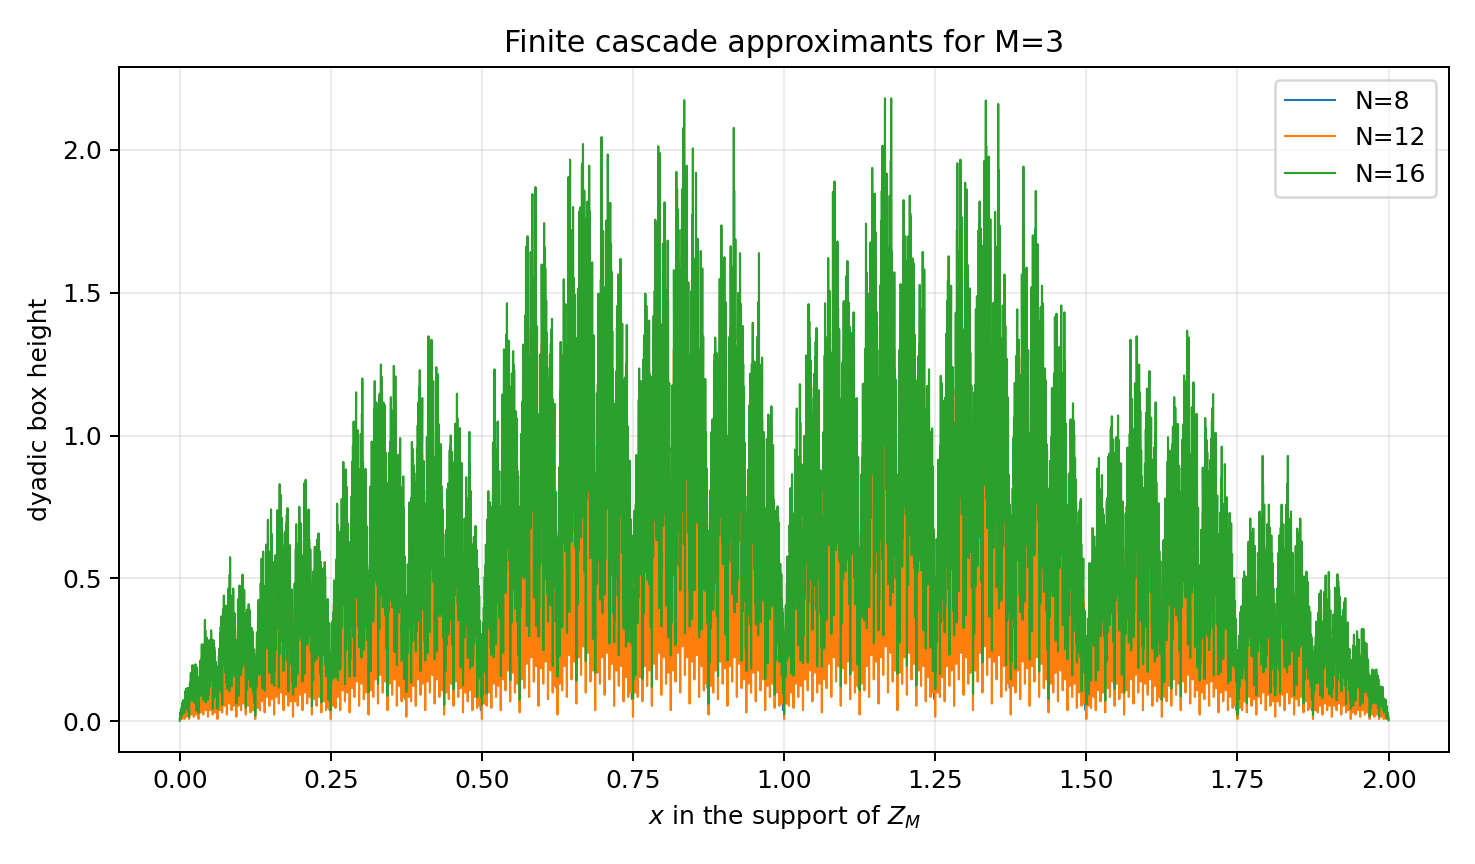
\includegraphics[width=0.94\textwidth]{figures/cascade_M3.png}
\caption{Dyadic box approximants for $Z_3$ at levels $N=8,12,16$.  The plot is a
visualization of finite atomic masses, not a claim that the singular limit has a density.}
\label{fig:cascade-M3}
\end{figure}

For $M=6=2\cdot3$, the uniform factor $\ReciprocalIntegerLaw{2}$ smooths the singular ternary core.  The
finite cascades rapidly agree with the continuous $C^0\setminus C^1$ density predicted by
\cref{thm:regularity}.

\begin{figure}[htbp]
\centering
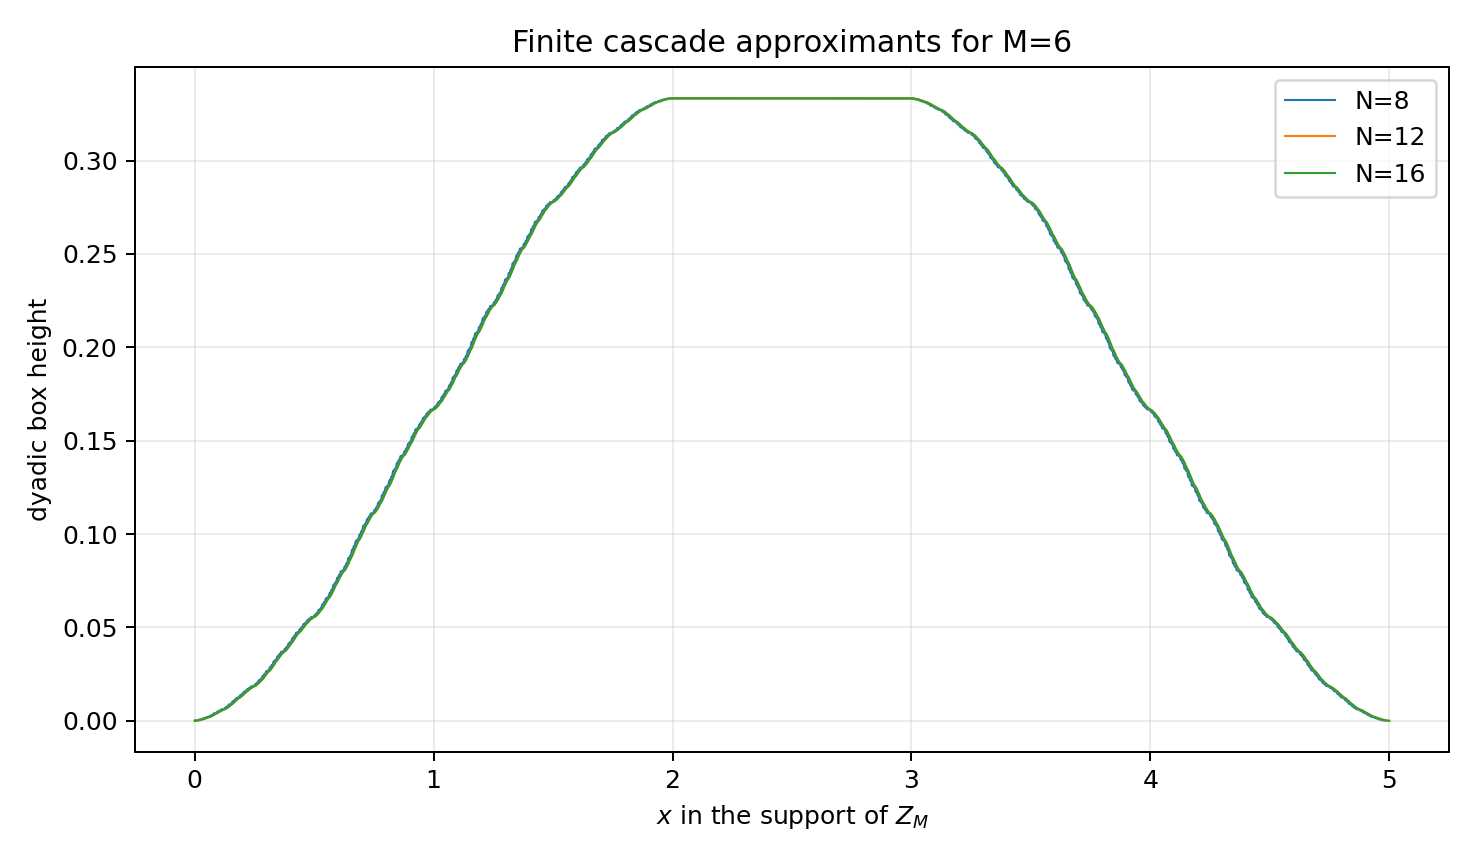
\includegraphics[width=0.94\textwidth]{figures/cascade_M6.png}
\caption{Dyadic box approximants for $Z_6$.  The near-coincidence of the three levels is
consistent with absolute continuity; the theorem, not the picture, identifies exact
regularity $C^0\setminus C^1$.}
\label{fig:cascade-M6}
\end{figure}

The exact output file \path{data/cascade_summary.csv} records maximum box heights and
$L^2$ energies.  For $M=3$, the maximum grows from approximately $1.3266$ at $N=8$ to
$2.4313$ at $N=16$, while for $M=6$ the profiles stabilize near the bounded continuous
limit.

\subsection{Endpoint phases}

The numerical phase
\begin{equation}
 \Omega_{M,N}(\theta)=2^{(\log_2M)\theta}
 \Probability(Z_{M,N}\le2^{-\theta})
 \label{eq:numerical-Omega}
\end{equation}
approximates the exact $\Omega_M$.  The $M=4$ curve is the constant $1/4$ from
\eqref{eq:Omega-power-two}; non-power cases show nonconstant phases, sometimes with small
amplitude.

\begin{figure}[htbp]
\centering
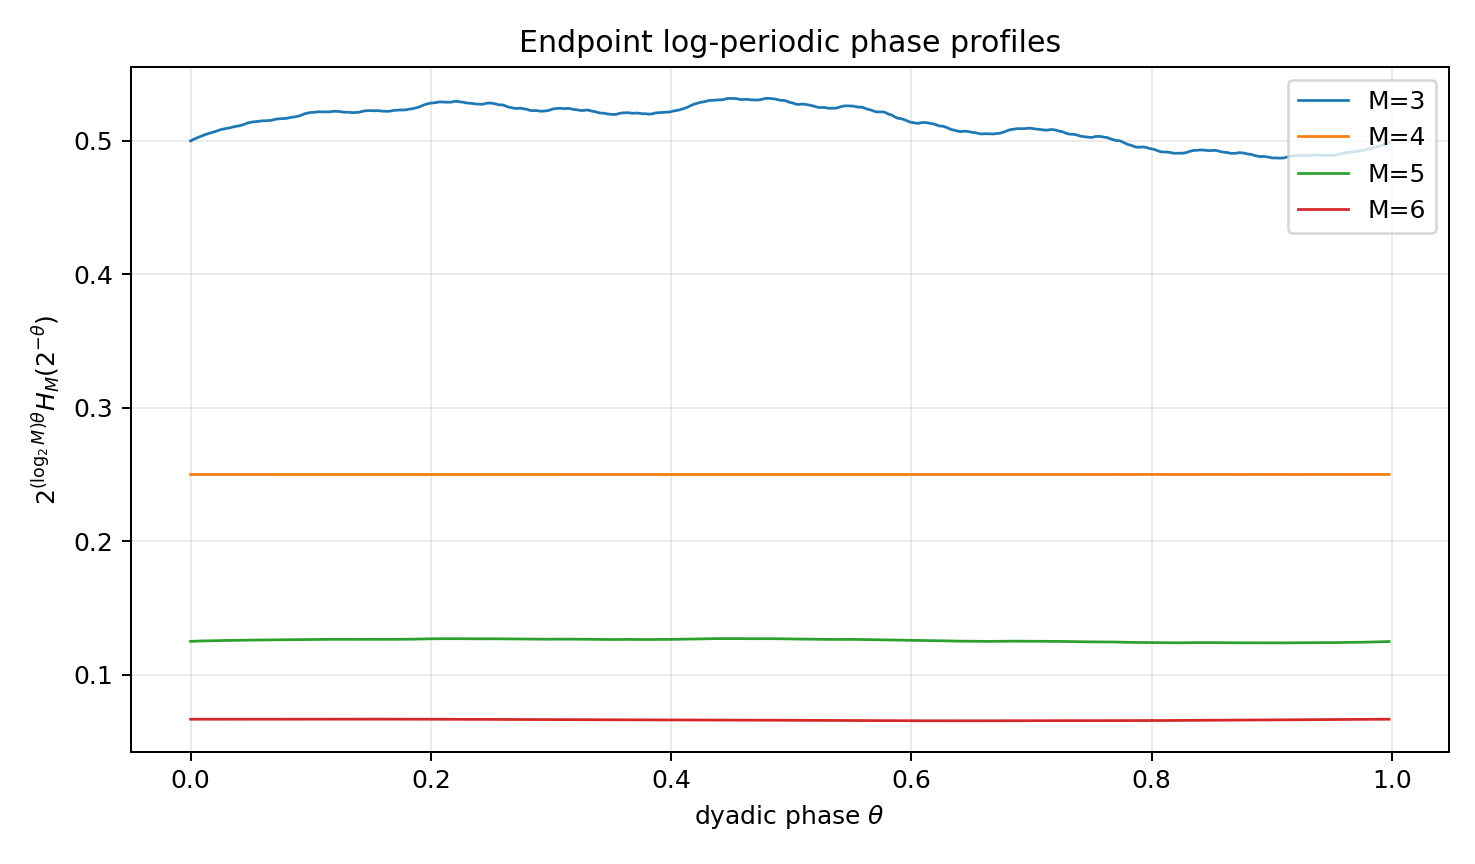
\includegraphics[width=0.94\textwidth]{figures/endpoint_profiles.png}
\caption{Finite-level endpoint phase profiles.  Power-of-two $M=4$ is exactly constant;
$M=3,5,6$ are nonconstant by \cref{thm:endpoint-rigidity}.}
\label{fig:endpoint-profiles}
\end{figure}

\subsection{Zero multiplicities and Fourier resonance}

\begin{figure}[htbp]
\centering
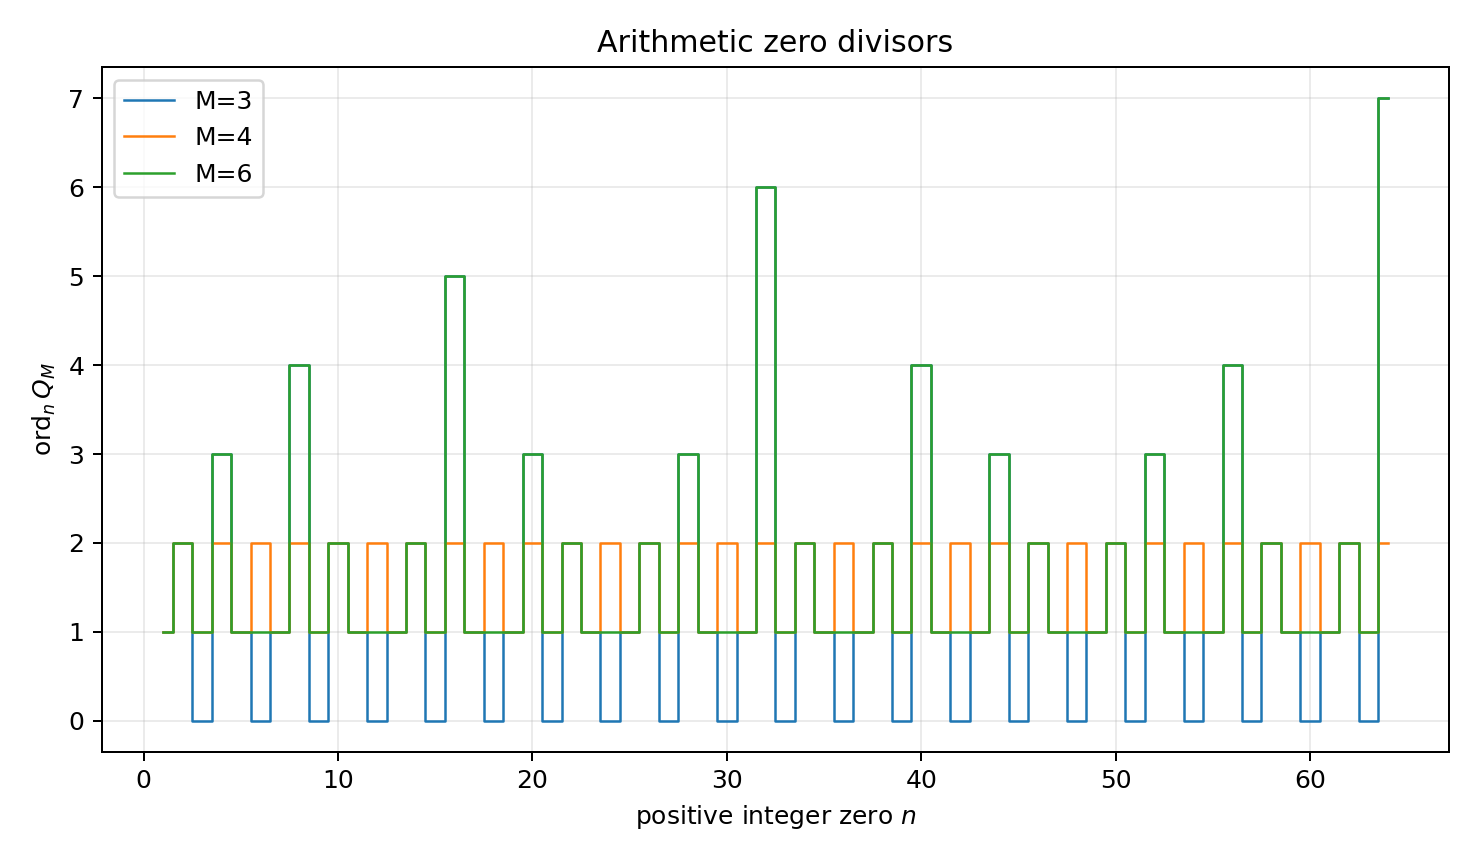
\includegraphics[width=0.94\textwidth]{figures/zero_multiplicities.png}
\caption{The first arithmetic zero multiplicities for $M=3,4,6$.  The $M=3$ divisor has
holes at multiples of $3$; even $M$ retain every integer zero.}
\label{fig:zero-multiplicities}
\end{figure}

The high-precision calculation gives
\[
 |Q_3(3\cdot2^k)|=0.083432097593273364307\ldots,
\]
\[
 |Q_5(5\cdot2^k)|=0.015632569447946944078\ldots,
\]
for every tested $0\le k\le10$, exactly as predicted by
\eqref{eq:nondecay-subsequence}.  The values and thirty-digit real parts are in
\path{data/odd_fourier_subsequence.csv}.

\subsection{Reproduction command}

From the extracted archive directory, run
\begin{lstlisting}[style=pseudo,language=Python,breaklines=true]
python experiments.py --output-dir .
\end{lstlisting}
The script regenerates all four PNG figures and all CSV/text data files.  Its final exact
checks raise an exception if either the Thue--Morse quotient identity or the Stern equality
fails.

\section{Mellin complex dimensions of the endpoint phase}
\label{sec:mellin-phase}

The exact edge law also has a short Mellin formulation.  Put
\begin{equation}
 \mathfrak M_M(s)=\int_0^{1/2}H_M(x)x^{s-1}\Differential x,
 \qquad
 B_M(s)=\int_{1/2}^{1}H_M(x)x^{s-1}\Differential x.
 \label{eq:endpoint-Mellin-def}
\end{equation}
The first integral converges initially for $\Re s>-\alpha_M$, while $B_M$ is entire.

\begin{proposition}[Endpoint Mellin lattice]
\label{prop:endpoint-Mellin}
The endpoint Mellin transform has the meromorphic continuation
\begin{equation}
 \boxed{
 \mathfrak M_M(s)=\frac{B_M(s)}{M2^s-1}.}
 \label{eq:endpoint-Mellin}
\end{equation}
Its candidate pole lattice is
\begin{equation}
 s=-\log_2M+\frac{2\pi\ImaginaryUnit k}{\log2},
 \qquad k\in\IntegerNumbers.
 \label{eq:endpoint-pole-lattice}
\end{equation}
The residue at a noncancelled pole is $B_M(s)/\log2$.  All nonzero-frequency poles cancel
if and only if $M$ is a power of two; for every non-power of two at least one nonreal pole
survives.
\end{proposition}

\begin{proof}
Use \eqref{eq:H-edge-scaling} and the substitution $u=2x$:
\[
 \mathfrak M_M(s)
 =\frac{2^{-s}}M\int_0^1H_M(u)u^{s-1}\Differential u
 =\frac{2^{-s}}M\bigl(\mathfrak M_M(s)+B_M(s)\bigr).
\]
Solving gives \eqref{eq:endpoint-Mellin}.  The pole lattice and residues are immediate.
To identify cancellations, decompose $(0,1/2]$ into dyadic shells and put
$x=2^{-(n+\theta)}$.  Up to a nonzero constant independent of $k$, the residue at
$s=-\alpha_M+2\pi\ImaginaryUnit k/\log2$ is the Fourier coefficient
$\int_0^1\Omega_M(\theta)\EulerE^{-2\pi\ImaginaryUnit k\theta}\,\Differential\theta$.  Hence a constant
phase cancels every nonzero-frequency pole, whereas a nonconstant continuous periodic
phase leaves at least one such pole.  Apply \cref{thm:endpoint-rigidity}.
\end{proof}

The zero-zeta lattice in \eqref{eq:dyadic-complex-dim} and the endpoint lattice in
\eqref{eq:endpoint-pole-lattice} differ by the real shift $-\log_2M$.  This is exactly what
one expects when a log-periodic function is multiplied by the leading power
$x^{\log_2M}$.  The result gives a precise bridge between the arithmetic zero divisor and
the inverse-function phase, while stopping short of claiming that their residues coincide.

\section{Conjectures and frontier problems}
\label{sec:conjectures}

The proved theorems leave several sharply formulated questions.  The conjectures below are
chosen to be falsifiable and computationally accessible.

\subsection{Fractional regularity from carry matrices}

For $M=2^rq$ with odd $q>1$, \cref{thm:regularity} determines the exact integer
regularity $C^{r-1}\setminus C^r$ but not the modulus of continuity of the highest
continuous derivative.  The carry recurrence \eqref{eq:cM-recurrence} yields a finite set
of transition matrices acting on overlap states.

\begin{conjecture}[Carry spectral radius controls sharp H\"older regularity]
\label{conj:carry-regularity}
For each odd $q>1$ there is an explicitly constructible finite family of nonnegative carry
matrices $\mathscr C_q$ such that the global H\"older exponent of the CDF of $\ReciprocalIntegerLaw{q}$, and
therefore the H\"older exponent of $g_{2^rq}^{(r-1)}$, is a simple logarithmic function of the
joint spectral radius of $\mathscr C_q$.  The same matrices determine the optimal Besov and
Sobolev exponents of $g_{2^rq}$.
\end{conjecture}

A practical route is to build automata for pairs of digit strings with equal or neighboring
binary values, then study collision energies
\[
 E_{q,N}=\sum_n c_{q,N}(n)^2.
\]
The growth exponent of $E_{q,N}$ should give the $L^2$ dimension and a first spectral
bound for regularity.  The included code already outputs finite-level energies.

\subsection{Infinitely rich endpoint phases}

\begin{conjecture}[No finite Fourier phase outside the spline cases]
\label{conj:phase-modes}
If $M$ is not a power of two, the periodic functions $\Omega_M$ and $\Psi_M$ have
infinitely many nonzero Fourier coefficients.  Equivalently, the endpoint Mellin transform
\eqref{eq:endpoint-Mellin} has infinitely many noncancelled nonreal poles.
\end{conjecture}

A stronger version would estimate the decay of the phase coefficients from the exact
regularity class in \cref{thm:regularity}.  This would turn the qualitative complex-dimension
picture into an explicit oscillatory asymptotic calculus.

\subsection{Dyadic arithmetic of the divisor CDF}

The original Fabius function takes rational values at dyadic arguments.  The digit measures
have even more explicit rational transition probabilities but also exact overlaps.

\begin{conjecture}[Rational dyadic values]
\label{conj:dyadic-rationality}
For every $M\ge2$, every integer $n\ge0$, and every integer $k$,
\begin{equation}
 H_M(k/2^n)\in\RationalNumbers.
 \label{eq:dyadic-H-conj}
\end{equation}
Moreover, these values can be computed by a finite carry Markov chain with a rational
transition matrix whose dimension is $O(M)$, and their reduced denominators satisfy an
explicit $M$-adic/$2$-adic valuation formula.
\end{conjecture}

For $M=3$, the boundary layers already involve Stern numbers.  A successful proof should
connect the finite Markov resolvent to Stern--Brocot or Calkin--Wilf matrices.

\subsection{Stern multifractality inside the singular $M=3$ divisor}

\begin{conjecture}[Stern spectrum]
\label{conj:Stern-spectrum}
The local dimension spectrum of $\ReciprocalIntegerLaw{3}$ is the Legendre transform of a pressure function
built from the standard two Stern matrices.  In particular, extremal local dimensions occur
at eventually periodic binary addresses and are logarithms of quadratic units divided by
$\log2$.
\end{conjecture}

The exact mass formula \eqref{eq:Stern-masses} makes this accessible: cylinder and
near-cylinder masses are controlled by products of the two matrices generating the Stern
recursion.  This appears to be a direct bridge from the Rvachev function to the metric theory
of the Calkin--Wilf tree.

\subsection{Mahler and natural-boundary rigidity}

\begin{conjecture}[Natural boundary for nonpower digit quotients]
\label{conj:natural-boundary}
If $M$ is not a power of two, the power series
\begin{equation}
 A_M(x)=\frac{T(x^M)}{T(x)}
 \label{eq:AM-quotient-conj}
\end{equation}
has the unit circle as a natural boundary and is transcendental over $\ComplexNumbers(x)$.  For
algebraic $0<|\xi|<1$, broad classes of values $A_M(\xi)$ are transcendental by a suitable
Mahler method.
\end{conjecture}

The power-of-two cases are exactly rational by \eqref{eq:A-power-two}; hence this conjecture
would add a function-theoretic member to the rigidity equivalences in
\cref{cor:rigidity-equivalences}.

\subsection{General integer bases}

For an integer base $b\ge2$, consider
\begin{equation}
 \Phi_b(z)=\prod_{n=0}^{\infty}\SincRad\!\left(\frac{\pi z}{b^n}\right).
 \label{eq:Phi-b}
\end{equation}
The same Dirichlet-kernel calculation constructs
$Q_{b,M}(z)=\Phi_b(z)/\Phi_b(z/M)$ for every integer $M$.

\begin{conjecture}[General-base divisor classification]
\label{conj:general-base}
For every integer $b\ge2$:
\begin{enumerate}
\item the only independent-copy scales of the $\Phi_b$ law are $0$ and $\pm1/M$;
\item if $M=b^rq$ with $b\nmid q$, then the divisor is singular continuous when $r=0$
and has exactly the regularity obtained by convolving the singular core with $r$ box laws
when $r>0$;
\item its zero-divisor zeta function is
\begin{equation}
 \mathcal Z_{b,M}(s)=(1-M^{-s})\frac{\zeta(s)}{1-b^{-s}};
 \label{eq:general-base-zeta}
\end{equation}
\item constant endpoint phase, finite sinc product, and $M=b^r$ are equivalent.
\end{enumerate}
\end{conjecture}

Most proof steps from the dyadic case transfer verbatim.  The remaining care concerns
composite-base valuations, knot separation, and the exact normalization of the generalized
atomic function.

\subsection{Legendre spectra and arithmetic preconditioners}

\begin{conjecture}[Divisor preconditioning of Legendre expansions]
\label{conj:Legendre-preconditioner}
For suitable $M=M(n)$, the triangular transfer \eqref{eq:Legendre-transfer} yields a
better-conditioned computation of the high-degree Legendre coefficient
$\Expectation P_n(X)$ than direct integration against $\RvachevUp$.  Powers of two
optimize symbolic
simplicity, while even non-powers optimize a tradeoff between compact spline smoothing and
nontrivial endpoint phase.
\end{conjecture}

A concrete experiment is to compare condition numbers of the lower triangular moment
matrices for $M=2^r$, $3\cdot2^r$, and prime $M$, using exact Bernoulli cumulants.  The
cocycle suggests prime-factor preconditioners assembled multiplicatively.

\subsection{Hybrid Lambert-$W$/divisor inversion}

The repository's inverse-Fabius expansion locates the extreme endpoint scale through the
$W_{-1}$ branch.  The divisor bracket \eqref{eq:F-inverse-bracket} is uniform but coarse
unless $M$ is large.

\begin{conjecture}[Hybrid certified inversion]
\label{conj:hybrid-inverse}
There is an adaptive scheme choosing $M$ and an innovation depth $k$ from the Lambert
phase of $p$ such that:
\begin{enumerate}
\item the Lambert-$W$ approximation provides a narrow initial interval for
      $\FabiusQuantile(p)$;
\item the quantile of $Y_{M^k}$ refines it with the rigorous radius $1/(2M^k)$;
\item $q=M^{-2}$ Richardson extrapolation reduces the Fourier/cascade work to
polylogarithmic complexity in the requested precision.
\end{enumerate}
\end{conjecture}

This would combine two presently separate parts of the corpus: all-orders endpoint
asymptotics and exact arithmetic self-similarity.

\section{A formalization and research program}
\label{sec:program}

\subsection{Current exact Lean adjacency and the quotient-family boundary}

At the merge-parent boundary above, two exact Lean modules are adjacent to this report's
zero-divisor program.  In
\path{Lean/FabiusFunction/GeneralizedZeroDivisor.lean},
\lean{Fabius.generalizedRvachevProduct_eq_zero_iff_int} gives the arithmetic
integer zero set for a generalized Rvachev product, while
\lean{Fabius.analyticOrderAt_generalizedRvachevProduct_int} gives its exact
order at every nonzero integer.  In
\path{Lean/FabiusFunction/ReciprocalIntegerGammaZeros.lean},
\lean{Fabius.geometricReciprocalGamma_inv_natCast_eq_zero_iff} identifies the
zero set of the geometric reciprocal Gamma function at every reciprocal-integer base.

These declarations are exact formal infrastructure, but they concern generalized Rvachev
products and geometric reciprocal Gamma functions.  They do not formalize the extension of
$Q_M=\Phi/\Phi(\mathord{\cdot}/M)$ through its removable singularities, its
characteristic-function interpretation, the reciprocal-integer convolution-divisor
classification, the quotient multiplicity formula, or the spectral zeta function in this
report.  Those claims remain manuscript-level results; the following list is a proposed Lean
development, not a crosswalk asserting that the quotient family is already formalized.

\subsection{Lean-sized theorem units}

The main arguments decompose naturally into formalization units:
\begin{enumerate}
\item prove the finite geometric-exponential identity \eqref{eq:Dirichlet-kernel};
\item construct $Y_M$ as an almost surely convergent bounded random series and identify its
characteristic function;
\item prove $\Phi=\Phi(\cdot/M)Q_M$ and the decomposition theorem;
\item use the existing formal zero-order theorem for $\Phi$ to prove the scale
classification and \eqref{eq:deltaM-general};
\item formalize the cocycle and its random-series coupling;
\item formalize the finite polynomial identity \eqref{eq:finite-TM-quotient};
\item derive cumulants as formal power-series identities before invoking analytic mgfs;
\item formalize the endpoint CDF scaling and power-of-two simplex volume;
\item isolate the measure-theoretic pure-type and regularity arguments.
\end{enumerate}
The first seven are comparatively low risk because they reduce to finite sums, entire
products already present in the repository, and integer valuations.  The exact regularity
statement needs the most measure/distribution infrastructure.

\subsection{Computational priorities}

The following experiments would most efficiently test the conjectures:
\begin{enumerate}
\item build minimal carry automata for $M=3,5,7,9$ and compute joint spectral radii;
\item estimate Fourier coefficients of $\Omega_M$ at high precision using exact recursive
CDF evaluation rather than finite histograms;
\item solve rational linear systems for $H_M(k/2^n)$ and search denominator patterns;
\item compute Legendre transfer matrices exactly through degree $100$ and compare
conditioning across factorizations of $M$;
\item test natural-boundary behavior of $A_M$ with Pad\'e tables and Mahler functional
relations;
\item compare odd singular and even smooth approximants in Wasserstein, Kolmogorov,
negative Sobolev, and total variation metrics.
\end{enumerate}

\subsection{Conceptual payoff}

The divisor family changes the usual viewpoint on $\RvachevUp$.  Rather than one special dyadic
infinite convolution, the Rvachev law becomes the terminal object of an arithmetic system of
innovation laws.  Prime factorization acts by convolution cocycles; $2$-adic valuation acts
as a regularity counter; odd factors generate singular cores; Thue--Morse signs invert the
positive digit counts; Bernoulli numbers diagonalize cumulants; Bell polynomials reconstruct
moments; and the inverse Fabius function is uniformly approximated by divisor quantiles.
This unifies several themes of the repository without repeating its existing endpoint,
Legendre, or $q$-series derivations.

\section{Conclusion}
\label{sec:conclusion}

The central object of this report is the entire quotient
\[
 Q_M(z)=\frac{\Phi(z)}{\Phi(z/M)}.
\]
A one-line Dirichlet-kernel identity turns it into a characteristic function, but the
consequences are unexpectedly broad.  The zeros of $\Phi$ classify all possible scales.
Prime multiplication becomes a convolution cocycle.  The odd part of $M$ determines a
singular continuous core, while the $2$-adic valuation counts smoothing boxes.  The same
arithmetic appears in zero multiplicities, a closed zeta function, torus aliasing, endpoint
log-periodicity, and finite digital polynomials.  At $M=3$, Stern's sequence enters as the
exact hyperbinary mass profile and is inverse-convolved by Thue--Morse signs.  As
$M\to\infty$, both smooth and singular divisors approach the Rvachev law at the exact
transport rate $1/M$.

The strongest proved frontier statements are therefore not isolated formulas but a
coherent arithmetic structure:
\[
 \boxed{
 \text{reciprocal scale}
 \Longleftrightarrow
 \text{integer divisor}
 \Longleftrightarrow
 \text{digit IFS}
 \Longleftrightarrow
 \text{zero-zeta Euler factor}.}
\]
The next decisive steps are to compute the carry spectra, resolve dyadic arithmetic of the
divisor CDFs, formalize the classification, and connect Mellin phase residues to the
repository's all-orders inverse and asymptotic machinery.

\appendix

\section{Proof supplements}
\label{app:proofs}

\subsection{The zero-zeta computation in one line}

For completeness,
\begin{align}
 \sum_{n\ge1}\frac{\TwoAdicValuation(n)}{n^s}
 &=\sum_{k\ge1}\sum_{2^k\mid n}\frac1{n^s}
 =\zeta(s)\sum_{k\ge1}2^{-ks}
 =\frac{\zeta(s)}{2^s-1},
 \label{eq:v2-Dirichlet}\\
 \sum_{n\ge1}\frac{1+\TwoAdicValuation(n)}{n^s}
 &=\frac{\zeta(s)}{1-2^{-s}}.
 \label{eq:m-Dirichlet}
\end{align}
Dilation by $M$ multiplies a Dirichlet series by $M^{-s}$, giving
\eqref{eq:zero-zeta}.

\subsection{Expansion at $s=0$}

Let $a=\log_2M$ and $h=\log M=a\log2$.  Then
\begin{equation}
 \frac{1-M^{-s}}{1-2^{-s}}
 =a\left(1+\frac{\log2-\log M}{2}s+\BigO(s^2)\right).
 \label{eq:A-at-zero}
\end{equation}
Multiplying by
$\zeta(s)=-\frac12-\frac12\log(2\pi)s+\BigO(s^2)$ gives
\eqref{eq:ZM-zero}--\eqref{eq:ZM-derivative-zero}.

\subsection{The finite-cascade coefficient recurrence}

If $C_{M,N}(x)=\sum_nc_{M,N}(n)x^n$, then
\begin{equation}
 c_{M,N+1}(n)=\sum_{j=0}^{M-1}c_{M,N}(n-j2^N).
 \label{eq:finite-coeff-recurrence}
\end{equation}
This is the exact update used in \path{experiments.py}.  It avoids floating-point
convolution and makes the checks of \cref{thm:TM-quotient} fully integral.

\section{Corpus coverage matrix}
\label{app:corpus}

\begin{longtable}{@{}>{\raggedright\arraybackslash}p{0.27\textwidth}>{\raggedright\arraybackslash}p{0.30\textwidth}>{\raggedright\arraybackslash}p{0.35\textwidth}@{}}
\toprule
Corpus component & Existing coverage used & Duplication avoided in this report\\
\midrule
\endfirsthead
\toprule
Corpus component & Existing coverage used & Duplication avoided in this report\\
\midrule
\endhead
Primary Fabius/Rvachev exposition & Fourier sinc product, random convolution, exact integer zero orders, Fabius/up normalization, moments and arithmetic background & No rederivation of the main endpoint asymptotic hierarchy, dyadic-value theory, or canonical primary exposition\\
\addlinespace
Thue--Morse atlas and frontier volume & Lacunary product $T(x)$, Prouhet identities, Mahler equations, finite-block calculus, Mellin/Dirichlet machinery & The new result is the positive digit quotient $A_M=T(x^M)/T(x)$ and its divisor interpretation, not another atlas of standard Thue--Morse formulas\\
\addlinespace
Exponents and $q$-series volume & Bell--Bernoulli expansions, $q$-binomial filters, general extrapolation machinery & Only the new integer parameter $q=M^{-2}$ and divisor approximants are developed; general $q$ identities are cited as infrastructure\\
\addlinespace
Inverse and sampling volume & Inverse endpoint expansions, Lambert $W_{-1}$, dyadic sampling, comb formulas & The uniform quantile bracket and divisor torus law are distinct global statements; the existing all-orders inverse expansion is not duplicated\\
\addlinespace
Representation frontiers & Legendre/Lagrange expansions, spline representations, multiresolution, polyphase structure & The report gives a new divisor-indexed triangular transfer, not a replacement derivation of the existing representation loops\\
\addlinespace
Frontier compilations & Spectral zeta, zero filtration, transport metrics, general atomic functions & The new zeta belongs to the quotient zero divisor and carries the Euler factor $1-M^{-s}$; odd singular approximants and complete scale classification were not found\\
\addlinespace
Frozen archive & Historical versions and provenance hashes & Used only to prevent an absorbed result from being mistaken as absent; repeated archived text is not recounted as new coverage\\
\bottomrule
\end{longtable}

\section{Archive contents and file map}
\label{app:file-map}

The repository package contains:
\begin{center}
\begin{tabularx}{\textwidth}{@{}p{0.56\textwidth}X@{}}
\toprule
Path & Purpose\\
\midrule
\path{Fabius_Rvachev_Reciprocal_Integer_Convolution_Divisors.tex} & complete LaTeX source\\
\path{Fabius_Rvachev_Reciprocal_Integer_Convolution_Divisors.pdf} & compiled report\\
\path{experiments.py} & commented reproducibility script\\
\path{figures/*.png} & four figures used in the PDF\\
\path{data/cascade_summary.csv} & finite-cascade maxima and $L^2$ energies\\
\path{data/zero_multiplicities.csv} & exact zero orders for sample $M$\\
\path{data/odd_fourier_subsequence.csv} & high-precision nondecaying Fourier values\\
\path{data/stern_hyperbinary_check.csv} & exact Stern coefficient comparison\\
\path{data/endpoint_profiles.csv} & plotted endpoint phase data\\
\path{data/experiment_summary.txt} & exact-check summary\\
\path{README.txt} & reproduction and compilation instructions\\
\path{SHA256SUMS} & live repository payload ledger\\
\bottomrule
\end{tabularx}
\end{center}

\begin{thebibliography}{99}

\bibitem{ProveItPrimary}
V. Reshetnikov,
\emph{Fabius Function and Rvachev Up}, living LaTeX exposition in the \repo\ repository,
\url{https://github.com/VladimirReshetnikov/ProveIt/tree/main/Analysis/FabiusFunction/docs/Fabius_Function_and_Rvachev_Up},
accessed 30 August 2026.

\bibitem{ProveItFrontiers}
V. Reshetnikov,
\emph{Semi-formalized research frontiers and draft manifest},
\url{https://github.com/VladimirReshetnikov/ProveIt/tree/main/Analysis/FabiusFunction/docs/semi-formalized-research-frontiers},
accessed 30 August 2026.

\bibitem{Arias1982}
J. Arias de Reyna,
\emph{An infinitely differentiable function with compact support: Definition and properties},
Rev. Real Acad. Ciencias Madrid \textbf{76} (1982), 21--38; English translation,
\url{https://arxiv.org/abs/1702.05442}.

\bibitem{Arias2018}
J. Arias de Reyna,
\emph{Arithmetic of the Fabius function},
Integers \textbf{18} (2018), Article A51,
\url{https://math.colgate.edu/~integers/s51/s51.pdf}.

\bibitem{Fabius1966}
J. Fabius,
\emph{A probabilistic example of a nowhere analytic $C^\infty$-function},
Z. Wahrscheinlichkeitstheorie verw. Gebiete \textbf{5} (1966), 173--174.

\bibitem{JessenWintner1935}
B. Jessen and A. Wintner,
\emph{Distribution functions and the Riemann zeta function},
Trans. Amer. Math. Soc. \textbf{38} (1935), 48--88,
\url{https://www.jstor.org/stable/1989728}.

\bibitem{DaubechiesLagariasI}
I. Daubechies and J. C. Lagarias,
\emph{Two-scale difference equations. I. Existence and global regularity of solutions},
SIAM J. Math. Anal. \textbf{22} (1991), 1388--1410.

\bibitem{DaubechiesLagariasII}
I. Daubechies and J. C. Lagarias,
\emph{Two-scale difference equations. II. Local regularity, infinite products of matrices,
and fractals},
SIAM J. Math. Anal. \textbf{23} (1992), 1031--1079.

\bibitem{DilcherEricksen2015}
K. Dilcher and L. Ericksen,
\emph{Hyperbinary expansions and Stern polynomials},
Electron. J. Combin. \textbf{22}(2) (2015), Paper P2.24,
\url{https://www.combinatorics.org/ojs/index.php/eljc/article/view/v22i2p24}.

\bibitem{Varju2022}
P. P. Varj\'u,
\emph{Self-similar sets and measures on the line},
in Proceedings of the International Congress of Mathematicians 2022, Vol. 4,
3620--3631,
\url{https://ems.press/content/book-chapter-files/33263}.

\end{thebibliography}

\end{document}
